%%% Clinic Statement of Work

%%% Clinic reports use the clinic class, which should be located
%%% somewhere in TeX's search path.

%%% For your ``statement of work'' (or ``work statement''), specify
%%% the ``proposal'' document-class option to the hmcclinic class.
\documentclass[book]{hmcclinic}

\setlength{\parindent}{24pt}

%%% The major difference between the statement of work and a midyear
%%% or final report is that the statement of work is typeset as an
%%% article, which means that the highest level of structural
%%% division available to you is section rather than chapter.

%%% There are also some changes in pagination styles and content
%%% that reflect the briefer nature of the proposal.  For example,
%%% in the longer reports, you use \frontmatter, \mainmatter, and
%%% \backmatter to separate some sections of the report from
%%% others.  In the statement of work, you don't need those
%%% commands, as no such division is necessary.

%%% Other packages needed by your document may be loaded here.
% \usepackage{url}              % For formatting URLs and other web or
                                % file references.
\usepackage[final]{pdfpages}
\usepackage{hyperref}
\usepackage{xcolor}
\usepackage{colortbl}
%%% Provide additional context around errors. 
\setcounter{errorcontextlines}{1000}

%%% Information about this document.

%%% I find it most useful to put identifying information about a
%%% document near the top of the preamble.  Technically, this
%%% information must precede the \maketitle command, which often
%%% appears immediately after the beginning of the document 
%%% environment.  Placing it near the top of the document makes it
%%% easier to identify the document, and keeps it out from getting
%%% mixed up with the real meat of the document.

%%% We use the same set of commands for specifying information about
%%% the people involved with the project that are used in the longer
%%% reports, so you can copy most of this information directly into
%%% your midyear and final reports.

%%% So, some questions.

%% What is the name of the company or organization sponsoring your project?
\sponsor{The Wenatchee AppleSox}

%% What is the title of your report?
\title{A Schedule Generator, Assessor, and Browser for the West Coast League}

%% Who are the authors of the report (your team members)?  (Separate
%% names with \and.)
\author{Julia Vendemiatti \and Omari Matthews \and Harry Aung \and Clayton North \and Cynthia Oh}

%% What is your faculty advisor's name?  (Again, separate names with
%% \and, if necessary.)
\advisor{Jim Boerkoel}

%% Liaison's name or names?
\liaison{Jose Oglesby \and Lauren Faux}

%% Did you have an outside consultant help you with this project?  Put
%% their names in the \consultant command.
%% \consultant{}

%%% End of information section.

%%% New commands and environments.

%%% You can define your own commands and environments here.  If you
%%% have a lot of material here, you might want to consider splitting
%%% the commands and environments into a separate ``style'' file that
%%% you load with \usepackage.

\newcommand{\coolcommand}[1]{#1 is cool.} % Lets everyone know that
                                % the person or thing that you provide
                                % as the argument to the command is
                                % cool.


%%% Some theorem-like command definitions.

%%% The \newtheorem command comes from the amsthm package.  That
%%% package is loaded by the class file.

%%% Note that these definitions have changed from the version in the
%%% sample report document by dropping the ``within'' argument.  See
%%% Gratzer's _Math into LaTeX_ or the AMS-LaTeX documentation for
%%% more details.

% \newtheorem{thm}{Theorem}
% \newtheorem{Theo1}{Theorem}
% \newtheorem{Theo2}{Theorem}
% \newtheorem{Lemma}{Lemma}


%%% If you find that some words in your document are being hyphenated
%%% incorrectly, you can specify the correct hyphenation using the
%%% \hyphenation command.  Note that words are separated by
%%% whitespace, as shown below.

  \hyphenation{ap-pen-dix wer-ther-i-an}


%%% The start of the document!

%% The document environment is the main environment in any LaTeX
%% document.  It contains other environments, as well as your text.

\usepackage{graphicx}

\begin{document}

%%% In a longer document (such as your midterm and final reports),
%%% you would have separate \frontmatter, \mainmatter, and
%%% \backmatter commands to define some large chunks of your
%%% document.  For the Statement of Work, which is a short document,
%%% we don't need these commands.

%%% Your Statement of Work begins with a title page.  The title page
%%% is formatted by commands in the document class file, so you
%%% don't need to worry about what it looks like -- just putting the
%%% \maketitle command in your document (and filling in the necessary
%%% information for the identification commands above) is enough.
\maketitle
%%% In a longer document or an article being submitted to a journal
%%% or conference, you would probably have an abstract that
%%% summarized the purpose of the document.  We don't need that for
%%% a Statement of Work.

%%% Similarly, in longer documents you would probably have commands
%%% to include a table of contents and lists of figures or tables.
%%% For a short document such as the Statement of Work, we don't
%%% need these commands.

%%% Table of Contents.
\tableofcontents
\newpage

%%% Content.

%%% Introduction
\chapter{Introduction}

The Wenatchee AppleSox is a collegiate summer baseball team that participates in the West Coast League’s North Division. The league spans the Pacific North West and parts of Canada. An integral part of every season is coming up with the game schedule, which, due to the large scale of the league, is not a simple task. There are multiple factors that have to be considered, such as the number of weekend home games each team gets or the maximum road trip length. Balancing these factors in the schedule is crucial for a good season. Not only does it balance the revenue that the teams generate from home weekend games, but it also protects the health and condition of the players by preventing travel weariness. 

Thus, the Wenatchee AppleSox have requested an interactive scheduling application that the league commissioner along with team owners can use to plan out the games for a season based on these factors. To adhere to the various preferences and requirements each team puts forth when taking part in a season, it is imperative that the scheduler allows exploration by the end user. Eventually, this tool could be expanded for use in other sports leagues, but the current focus is on the West Coast League. 

The owner of the Wenatchee AppleSox requested a computational solution that generates schedules for the West Coast League. Currently, a single individual is responsible for creating the schedule for the league each year. The whole process is extremely labor intensive and time consuming, requiring several weeks to create a potential schedule that is suitable for all of the teams in the league. Automating this process would take the majority of the load off of the commissioner in creating these schedules as well as reduce the amount of time required to generate a suitable schedule.

%NOTE: Not sure if this paragraph belongs here? we can talk about this stuff in our final product

%Our computational solution is composed of a system that implements a scheduling algorithm through an interactive application. The back-end consists of a scheduling algorithm, which takes in as input all the various factors being considered, such as distance and travel between stadiums, or home versus away games, and generates a valid schedule. The front-end implements an intuitive interface which allows users to interact with the scheduling algorithm by inputting constraints for the desired schedule. An interactive application would be ideal such that various parameters can be changed throughout the seasons.

The owner of the Wenatchee AppleSox has previously explored potential computational solutions for generating schedules. However, these solutions had one or more of three issues: poor user interface, lack of desired functionality, or slow run-times and turnaround. More specifically, the slow turnaround interferes with the iterative nature of finalizing a league schedule. Any prospective schedule has to be evaluated and approved by all the teams, and often goes through multiple rounds of changes before being finalized. A slow turnaround at each of these iterations of the schedule makes a computational solution unusable, as a schedule must be decided within a certain time-frame every season. The closest computational solution to what the owner wanted, created by John Hopkins, had exactly this problem. The schedule would take weeks to be generated and optimized, which, while theoretically optimal, could not adapt to the more human needs and preferences of the teams fast enough compared to the commissioner.

Thus, our goal was to create a product that addressed all three issues, a more intuitive schedule generator with all the desired functionality that supports the iterative nature of the process.

\section{Objectives}
In the statement of work, two main goals were identified:
\begin{enumerate}
 \item A minimum viable product (MVP) that solves the tournament scheduling problem  with the basic requirements.
  By the end of the fall semester, our team promised to deliver a minimum viable product (MVP) which includes:
 \begin{enumerate}

 \item All hard requirements added to the solver 
 \item Wireframes for web application
 \item Initial integration of front and back-end
 \item Functional web application for parameter inputs
 \end{enumerate}
 \item The final product that solves the tournament scheduling problem meeting all of the objectives listed in the objectives section.

    
\end{enumerate}

Our goal for the semester was to polish the MVP we created last semester by improving the user interface and by making the solver more accessible. More specifically, we spent this semester focusing on replacing our solver with one that better met the requirements of our liaisons, creating different user interfaces that would be useful for a wide variety of users, and diligently documenting these processes.  



\chapter{Technology}

The high level organization of the work into our user interface and web application is as follows. First, we thought about how we wanted to represent the scheduler's requirements. Then, we researched the tools we could use to build the web app and began wire-framing. From there, we started building a skeletal website and adding functionality for user inputs. Once we had a basic website working, we began integration so that the user input could be passed to our solver.

In the initial brainstorming stage, we considered various factors that influenced how we wanted to represent the scheduler's requirements on the website. At first, we spent a lot of time on how we wanted to translate the input values because there were a wide variety of parameter types we were taking into the schedule generator. After careful analysis of our input parameters we realized that we had roughly three main types of inputs: integer values, calendar dates, and text strings. This would cover all types of inputs that we needed to create. After deciding this, we set off to build each of these input forms as individual components we could reuse and customize. The next part of our work was figuring out how to translate the input value into a call to the back-end for the solver to return a schedule to us. A lot of this work was dependent on what tools we would use to connect the front and back-end which in information that can be found below. 

From the various tools we researched to build the web app, we settled on using React JS to build the website and Flask to run a Python script that does the schedule computation.  At one point, we considered using Typescript instead of Javascript, because Typescript is better for type safety. However, Javascript was more compatible with React which had many pre-existing libraries that would help build a front-end with cleaner user interface. In addition, React JS had a lot of readily provided tutorials and documentation that made the learning process much easier for us. Then, we chose to use Flask because it seemed to be the most popular tool to connect a React front-end and Python back-end program together, which meant that it would have the most documentation for us to reference. There were other options such as Django which is better fitting for more complex full stack web framework, but for our usage, we found that Flask was a more lightweight and simple tool. After setting all of this up, we went into work to figure out how to send the inputs to the solver and display the results of the solver in a user friendly way on the page. Essentially, the front-end React program sends an array of the values from the input form to the back-end solver which then runs based on those inputs. Once the solver is done running, it outputs a string which is then parsed in the front-end and displayed in a slot view. 

\begin{figure}[ht]
\begin{center}
\fbox{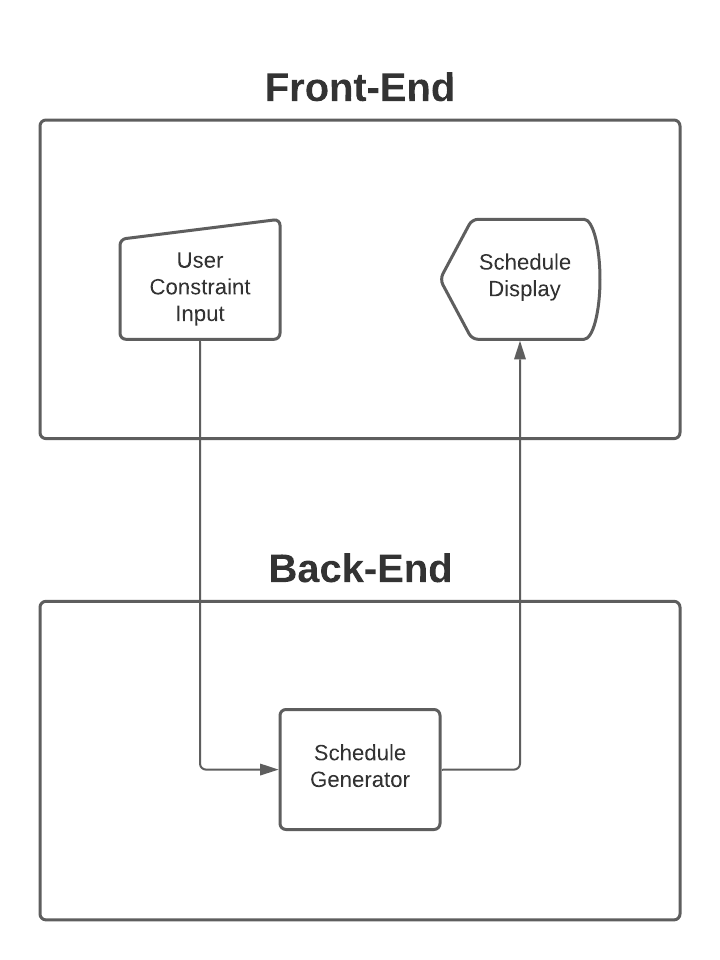
\includegraphics[scale=0.5]{simple_flow.png}}
\caption{General flow of information through the web application}
\end{center}
\end{figure}

% For the web app interface, we used ReactJS, an open-source JavaScript library for building user interfaces or user interface components. We used Javascript to build our website. With Reacts reusable components we were easily able to create the inputs to be put into our schedule. We also felt ReactJS had many pre-existing libraries that would help build a cleaner user interface. Additionally, ReactJS had a lot of readily provided tutorials and documentation that made ReactJS easier and quicker to implement into our web app. We also chose to use Flask, a web framework written in Python, because it is commonly used in conjunction with a ReactJS front-end and a Python back-end program. There was also a lot of documentation and online resources for using Flask and ReactJS together. For our usage we found Flask was lightweight and simple to setup. Together, the front-end ReactJS sends an array of the values from the input form to the Flask back-end to run through the scheduler, then Flask returns the schedule to React to be displayed. 

For deployment of our web app, we used Heroku, a container-based cloud platform used to deploy web applications. We decided to use Heroku because it worked well with React, Node Package Manager (NPM, used to install React), and Flask. Previously we had spent time trying to deploy with PythonAnywhere, but found that it was not compatible with NPM, hence we decided to switch to Heroku. 

For finding a schedule, we built a Python framework that made use of an existing integer linear programming solver, as it allowed us flexibility in approaching the problem, and saved us time from implementing the under-lying algorithms. Previously in the project we created our solver using IBM’s CPLEX Optimization Studio. However, due to the cost and accessibility, we decided to shift to an open source solver library. After much research we decided to use Python's Mixed-Integer Linear Programming library (MIP). MIP is a free, open source tool with plentiful documentation making the transition from CPLEX to MIP easier than expected. Our command line interface also used Excel to output schedules, making use of openpyxl, a Python library used to read and write Excel files.


\chapter{Development Process}

\section{Formulation of the Integer Linear Problem}
In the initial stages of the project, we researched various types of constraint satisfaction algorithms that we could apply to schedule generation. We encountered a paper by Dur´an, Guillermo, and Mario Guajardo entitled \textit{Scheduling the Chilean Soccer League by Integer Programming} (2007), which proposed integer linear programming (ILP) to find a solution for sports tournament scheduling. 

In essence, for the ILP approach, we create variables for each possible game and date. Then, we formulate integer equations, called constraints, for each requirement that needs to be satisfied. For example, to ensure that each team plays only once per day, we sum the games each team plays in a day and state that it needs to be equal to one. All of the requirements that the user has for the schedule is represented as and formulated as one of these constraints. This makes up a majority of the desired functionality that other computational solutions were lacking, which is the ability to satisfy these requirements. More detail about how these constraints work can be found in Appendix A, the Jupyter notebook explaining our solver.

\subsection{Solvers}
After formulating all the requirements into a linear equation, we chose to use an existing ILP solver library as it saved us time from implementing the underlying algorithms, and allowed us flexibility in approaching the problem. In the first semester, After researching the existing solvers, we found two main candidates: CPLEX and Gurobi. As they both had the speed and power we desired and are both accessible through Python, the deciding factor was IBM’s academic license for CPLEX that allowed us to develop and test our model for free until we decide to deploy or distribute. After deciding on CPLEX, we began implementing our ILP formulation as a CPLEX model, which CPLEX would then solve. Soon after, we found a simple open-source tournament scheduler provided by IBM as one of the examples on how to use CPLEX, which we iterated on to build the solver.

However, after further conversation with our liaisons during the second semester, we realized that CPLEX would no longer be a viable tool because of its cost and the fact that it is not open-source. Thus, we decided to move forward with an open-source python library, MIP. Our biggest concern of cost was no longer a worry with MIP. More importantly, open source programs allow for public collaboration such that they are improved continuously over time and are reliable due to large user bases. Although it is not as fast as CPLEX, it was fast enough to still produce a schedule in under a minute given an example set of requirements from our liaison -- this was fast enough for our purposes. We spent the following weeks performing the migration from CPLEX to MIP.

Luckily, the migration process was more straightforward than expected. We changed the pre-existing solver code to be object oriented and translated our constraints to fit MIP. Let us take a look at an example of an implementation of a requirement that was changed in this process. Figure 3.1 is a snippet of one of the requirements implemented for the CPLEX solver. This constraint ensures that each team only plays once and there are no duplicates. 

\begin{figure}[h]
    \centering
    \fbox{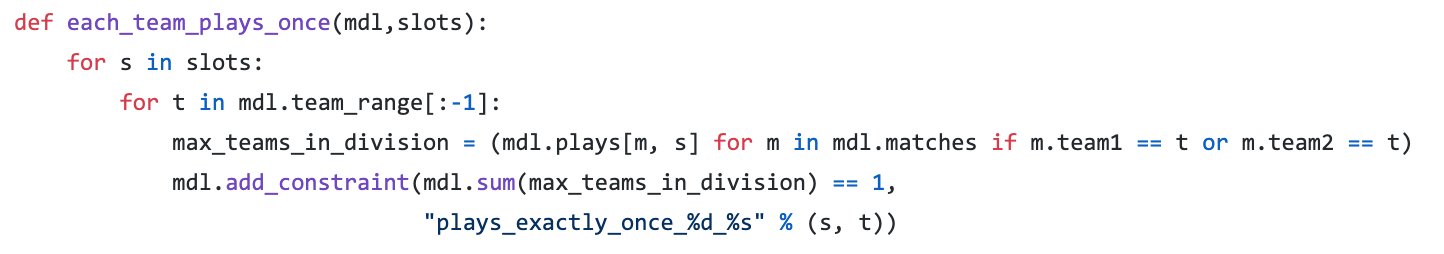
\includegraphics[scale=0.5]{Screen Shot 2021-03-01 at 2.39.57 PM.png}}  
    \caption{CPLEX Compatible “each\_team\_plays\_once” Implementation}
\end{figure}

Then, in comparison, we have Figure 3.2, which is the new code that we have written this semester. The general structure of using the nested for loops to traverse through the slots is retained in this code. However, there are a few differences as well. First, we see that the MIP version of the code no longer takes in external parameters because self contains all of the needed information with object oriented code. Second, we utilize BYEs in this code to check whether a team is playing. Overall, due to the generally similar structure, the code translation process went smoothly. 

\begin{figure}[h]
    \centering
    \fbox{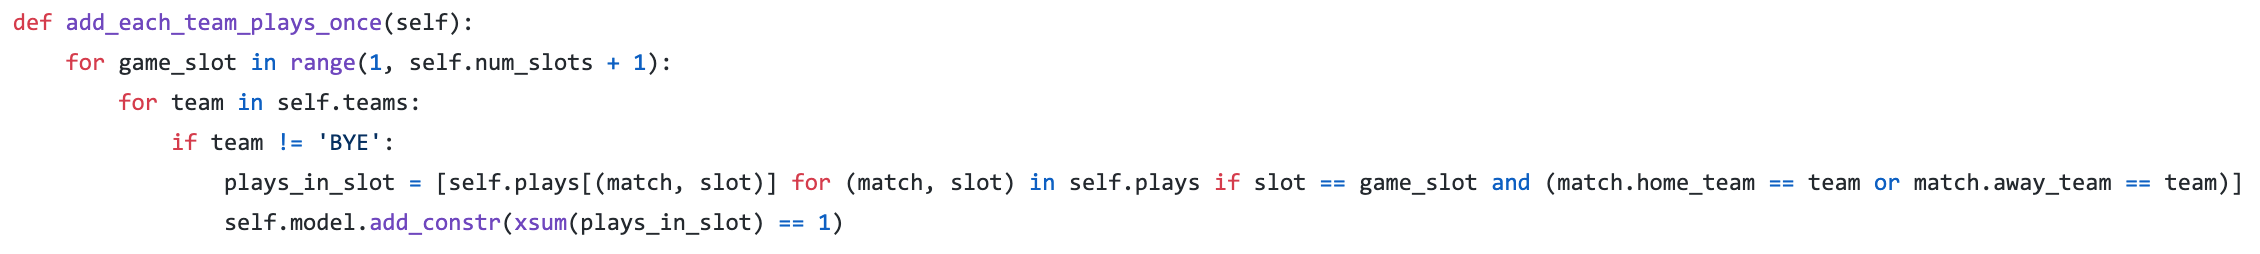
\includegraphics[scale=0.3]{Screen Shot 2021-03-01 at 2.41.07 PM.png}}  
    \caption{MIP Compatible “add\_each\_team\_plays\_once” Implementation}
\end{figure}

A lot of the translation process was aided by public resources from MIP and CPLEX. We now have a sport schedule solver that runs purely using MIP.




\section{Creating the User Interfaces}
When we started this project, we knew we wanted a graphical way of interfacing with our solver so that it would be intuitive for end users. That is, people who may not be familiar with the inner workings of our solver. This is the main purpose of the web application which we created in the fall semester. We made use of text boxes, counter inputs, list option inputs, and a visual matrix, all of which a user can interact with. In addition to the components themselves, we worked on concise, clear explanations and examples for each input type to help walk the user through the entire input form.

We also created a command line interface in the second semester in consideration of developers who would be making use of this product. Thus, our final product ended up having two different user interfaces to cater to our wide array of users. 

\subsection{Addition of Who-Plays-Who Matrix}
Initially, the liaisons suggested we take as input, a list of teams and given divisions, with a stretch goal being able to determine divisions just from a list of teams. The division a team was in determines which teams and how many times they would play. Some work was done in trying to handle multiple divisions, asymmetric divisions, and division cross-play. However, in early November we transitioned from this heuristic of divisions determining which teams and how many times a team would play, to a more explicit "who-plays-who" matrix (WPW). The WPW encodes the information of how many times each team each one plays every other team, both home and away throughout the season. This was done in response to new feedback from the liaisons, and so our scheduler no longer takes in divisions as input, but translates a WPW into the corresponding constraints for our model.

\subsection{Design and Layout of Web Application}
Because the web application is user facing, it is important to get feedback on the design and usability of the website from potential users. This semester, our liaisons introduced us to the commissioner of the West Coast League. During this session, he and our liaisons gave us valuable feedback about the usability of our website. Our biggest takeaway from the meeting was that there was too much information displayed to the user at once. As you can see in figure 3.3, all of the inputs for each constraint are displayed at the same time. Our liaisons pointed out that this could be confusing to a potential new user who does not know where to start. In order to mitigate the potential confusion, we decided to switch to a wizard-based approach. Each constraint that the user can input into the solver has its own dedicated page on the wizard. The user is able to navigate through these pages using a "previous" and "next" button, as shown in figure 3.4.

\begin{figure}[h]
    \centering
    \fbox{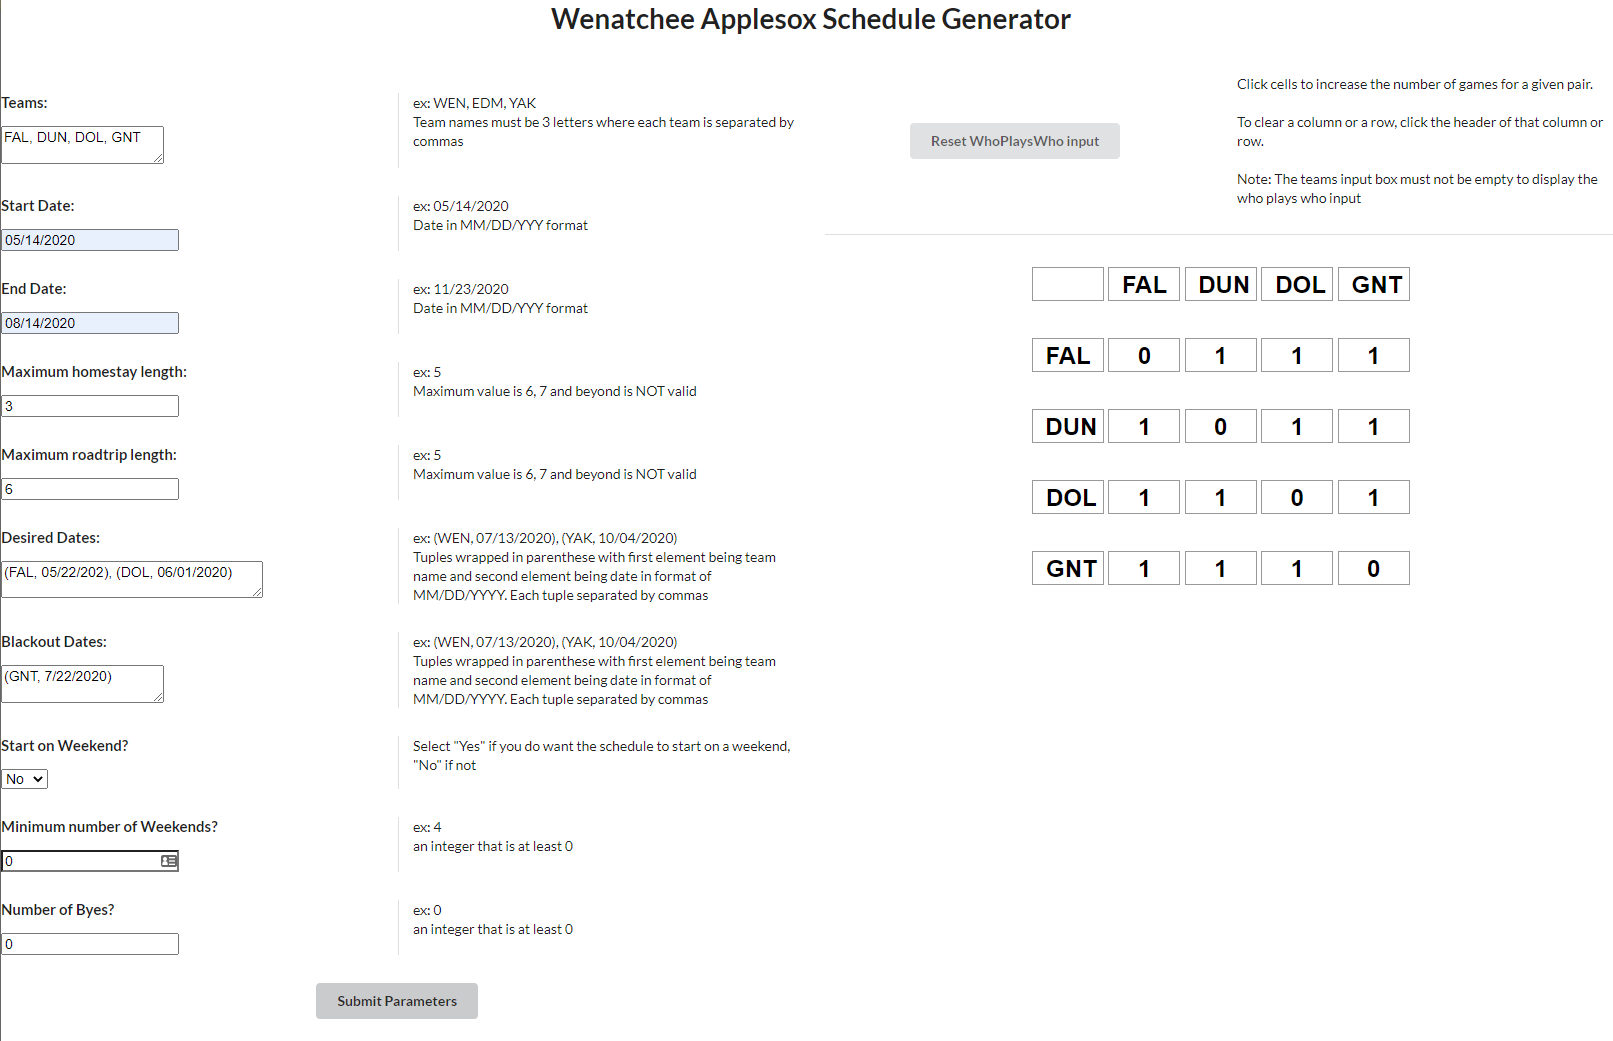
\includegraphics[scale=0.16]{front-end-input-form.png}} 
    \caption{Original Input Form Design}
\end{figure}
\begin{figure}[h]
    \centering
    \fbox{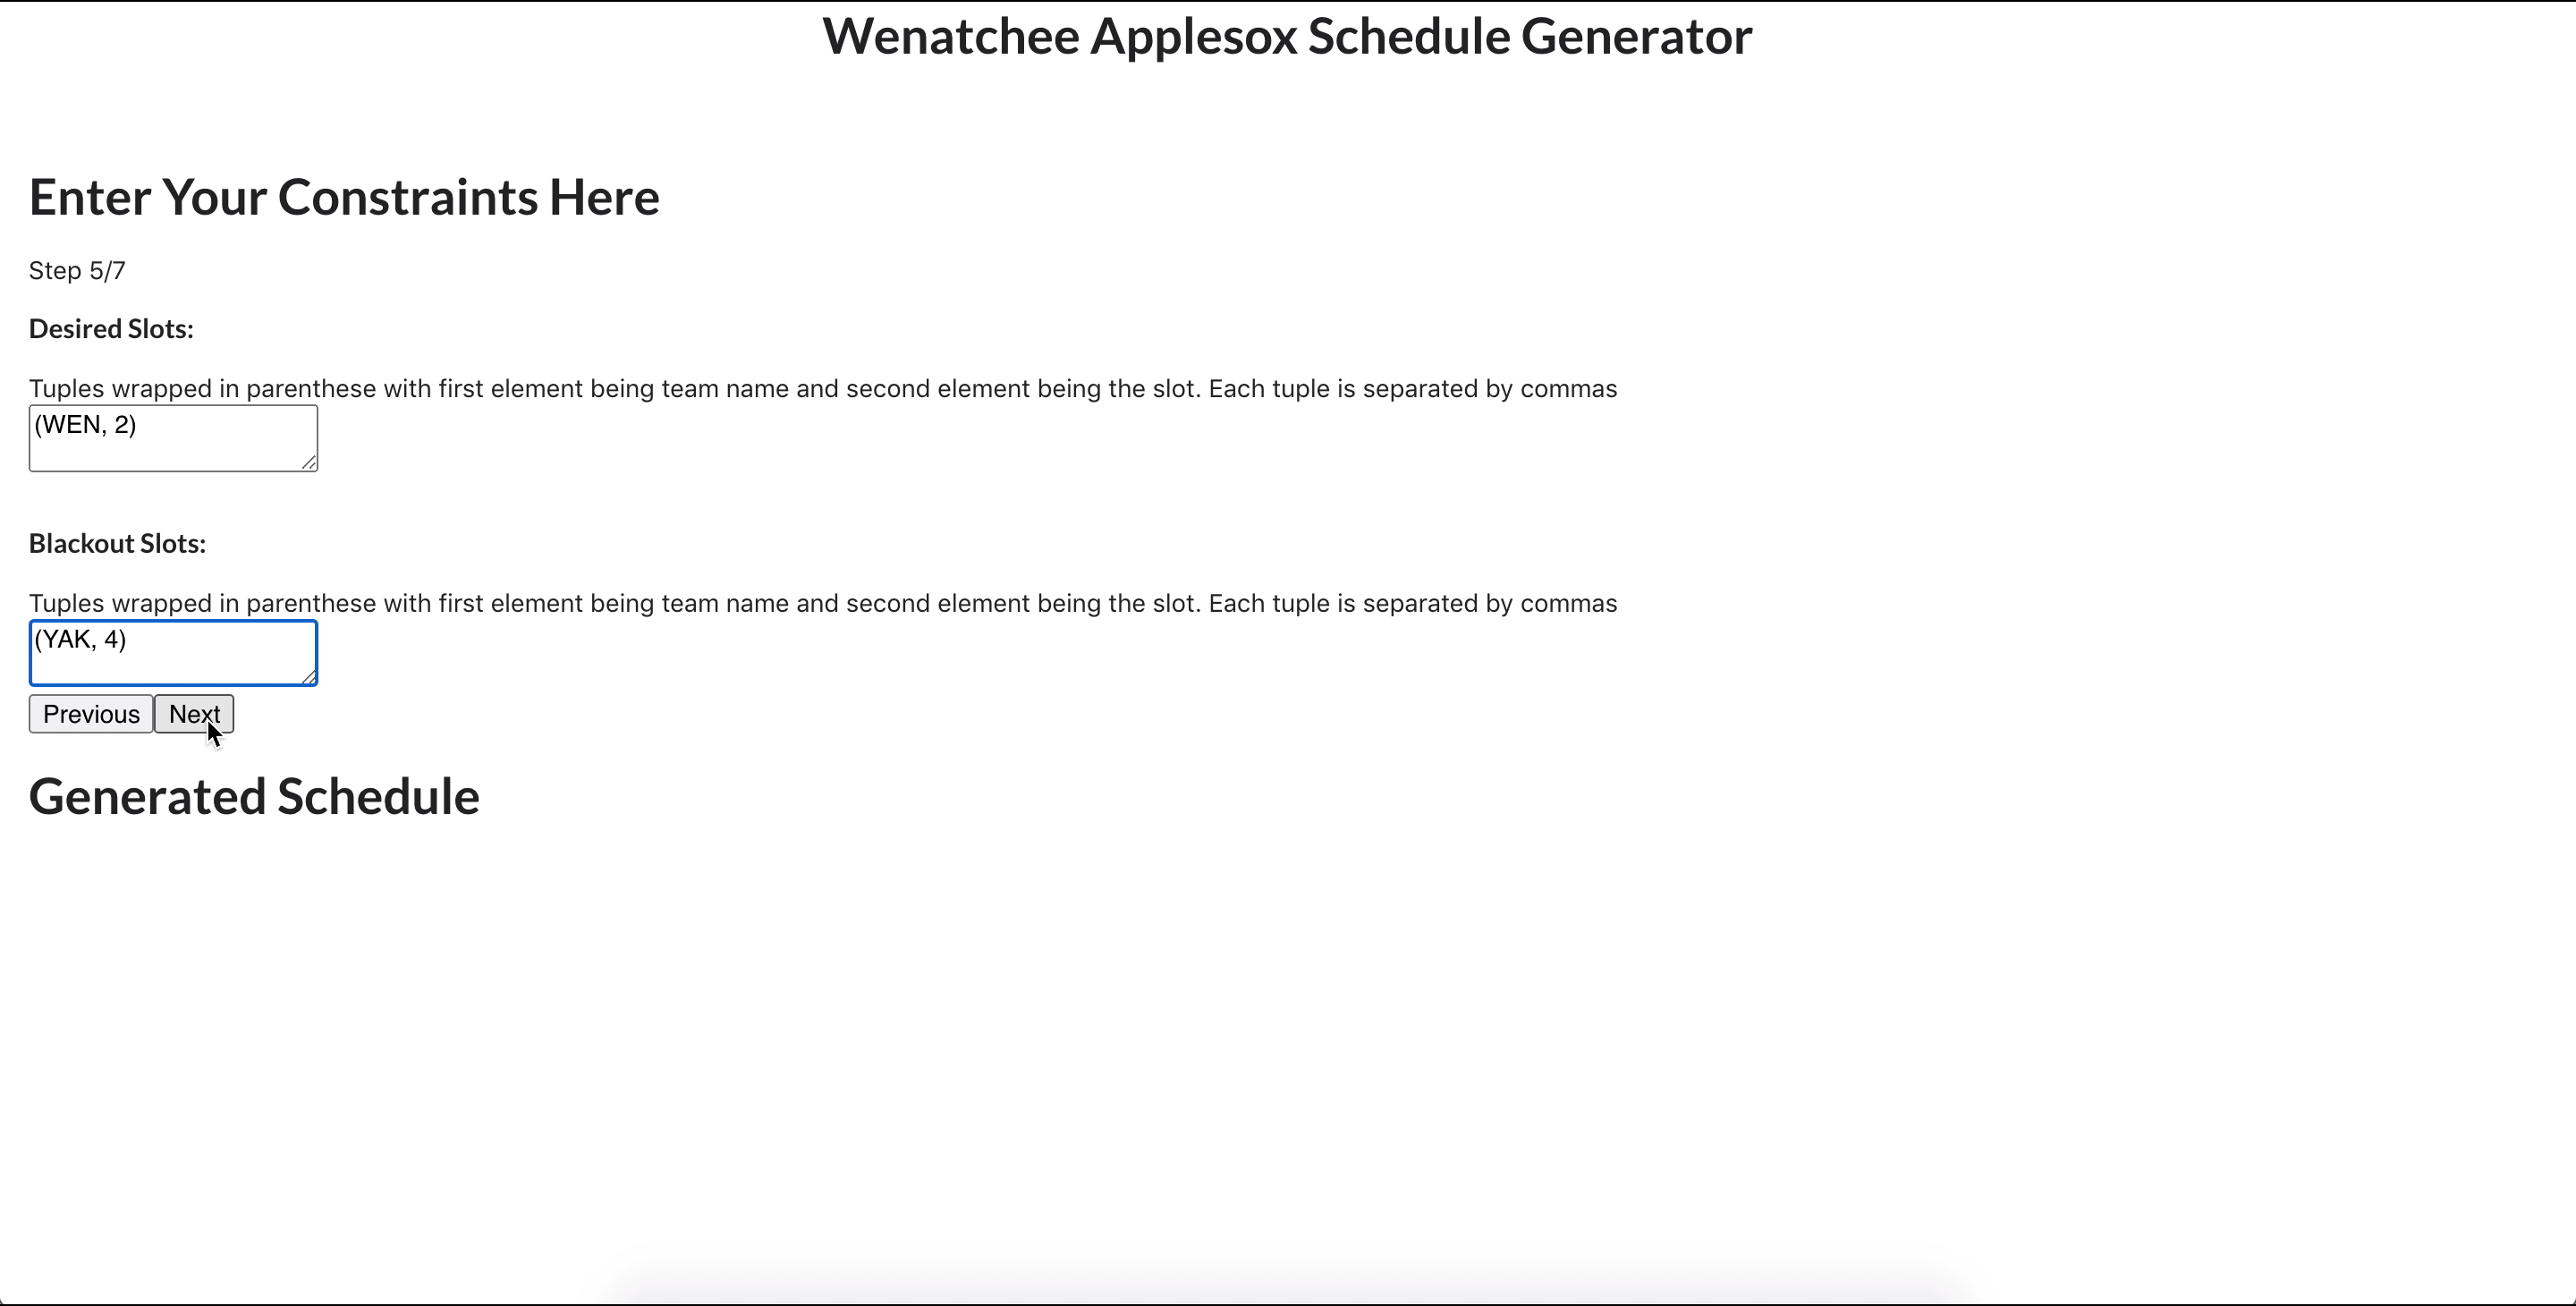
\includegraphics[scale=0.16]{Screen Shot 2021-05-07 at 1.28.43 AM.png}} 
    \caption{Wizard-Based Input Form Design}
\end{figure}

\subsection{Command Line Interface}
As we moved towards a more open source mindset, we had to consider a new set of users -- developers. This prompted us to create a command line interface. With it, developers could pre-define constraints and feed them to the solver without having to go through the input wizard of the web app every single time. The main purpose of the command line interface would be to streamline the development process by allowing developers to test multiple different inputs without the overhead of a graphical interface. 


 \section{Deployment}
While collection of the user input is handled on the front-end via the user interface, the back-end handles generating the schedule with the requirements defined in the user input as well as sending the generated schedule (and any other relevant information) back to the user interface to be displayed. The back-end makes use of \textit{Flask}, a micro web framework written in Python. For the back-end, Flask is used to define two HTTP requests: a POST request to send the user inputs from the front end to the Flask server where they are then inputted into the solver and a GET request to retrieve the solved schedule and other information from the Flask server. 

 %% Final Product - 
 \chapter{Final Product}

\section{Use}
Our final product will be used by the Wenatchee Apple Sox and the West Coast League to generate a schedule for their summer season. At the beginning of the project, a single individual was responsible for creating the schedule for the league each year. The whole process was extremely labor intensive and time consuming, requiring several weeks to create a potential schedule that is suitable for all of the teams in the league. Our final product allows one person to quickly and easily input the List of Teams, Who-Plays-Who Matrix based on input teams, Start Date, Maximum Homestay Length and Maximum Away Length, Desired Slots and Blackout Slots, Starts on Weekend and Minimum Number of Weekends, and Number of BYEs into a user interface inside of a website to create a schedule in a matter of minutes. Our final product also contains a simpler command line version which allows the user to generate a schedule locally by inputting two requirement files into a python script that we created; that way, the user can input requirements pre-defined in files instead of having to go through the user interface. Our command line version also allows for an easy way to create a color coded schedule in an Excel format.  

\section{Solver}
The solver is implemented as a Python class which makes use of the Model class from the MIP library, and previously a similar class from CPLEX. This Model class comes with the methods and functions needed to model our problem and solve that model to give us a schedule. Our class takes in the requirements of the season as input and has functions to translate those requirements into ILP constraints. Both the user interface and command line interface are integrated with the Python file containing this class to create an object of this class.

The problem is modelled as a 2-dimensional binary matrix. One dimension of the matrix is all possible matches, every combination of home and away team. The other dimension is the number of slots in the season. We define a variable as an entry in this matrix, with a 1 representing that match being played on that date, and 0 meaning otherwise. An example of accessing a variable in the matrix would be
$$\texttt{matrix[match:(home:'WEN',away:'CMS'),slot:5]},$$
which represent the Wenatchee AppleSox playing the Claremont-Mudd-Scripps team as their fifth series in the season.

The requirements for the season are implemented by iterating through the matrix and adding mathematical equations to be enforced, called constraints in CPLEX and MIP, on these variables. For example, to implement the blackout date requirement that the Wenatchee AppleSox can't play at home on slot 3, the solver adds the constraint
$$ \texttt{matrix[match:(home:'WEN',away:Team],slot:3] == 0},$$
to every variable in the matrix that matches that format. Requirements such as maximum road-trip length involves adding multiple variables together and checking that the sum is less than the max allowed.

The solver then populates the matrix with 0s and 1s in a way such that all constraints are satisfied, and we parse that matrix into a final schedule. Further documentation on how this solver works in a Jupyter notebook, which is included in the Appendix.



\section{Web Application}
Our final user interface for the web application is in the form of seven consecutive pages in which the user navigates through to put in different input values. The order is as follows: List of Teams, Who-Plays-Who Matrix based on input teams, Start Date, Maximum Homestay Length and Maximum Away Length, Desired Slots and Blackout Slots, Starts on Weekend and Minimum Number of Weekends, Number of BYEs. Some factors are put on the same page due to the size of the input component. In total, we use string input type, matrix input type, list option input type, integer count input type for the different factors. To navigate between the different pages of the input form, the user can use the "Previous" and "Next" button at the bottom of each of the pages. Below are figures of two of the input pages out of a total of seven, Figure 4.1 and Figure 4.2. It shows a matrix input for the Who-Plays-Who matrix and counter input type. 

\begin{figure}[h]
    \centering
    \fbox{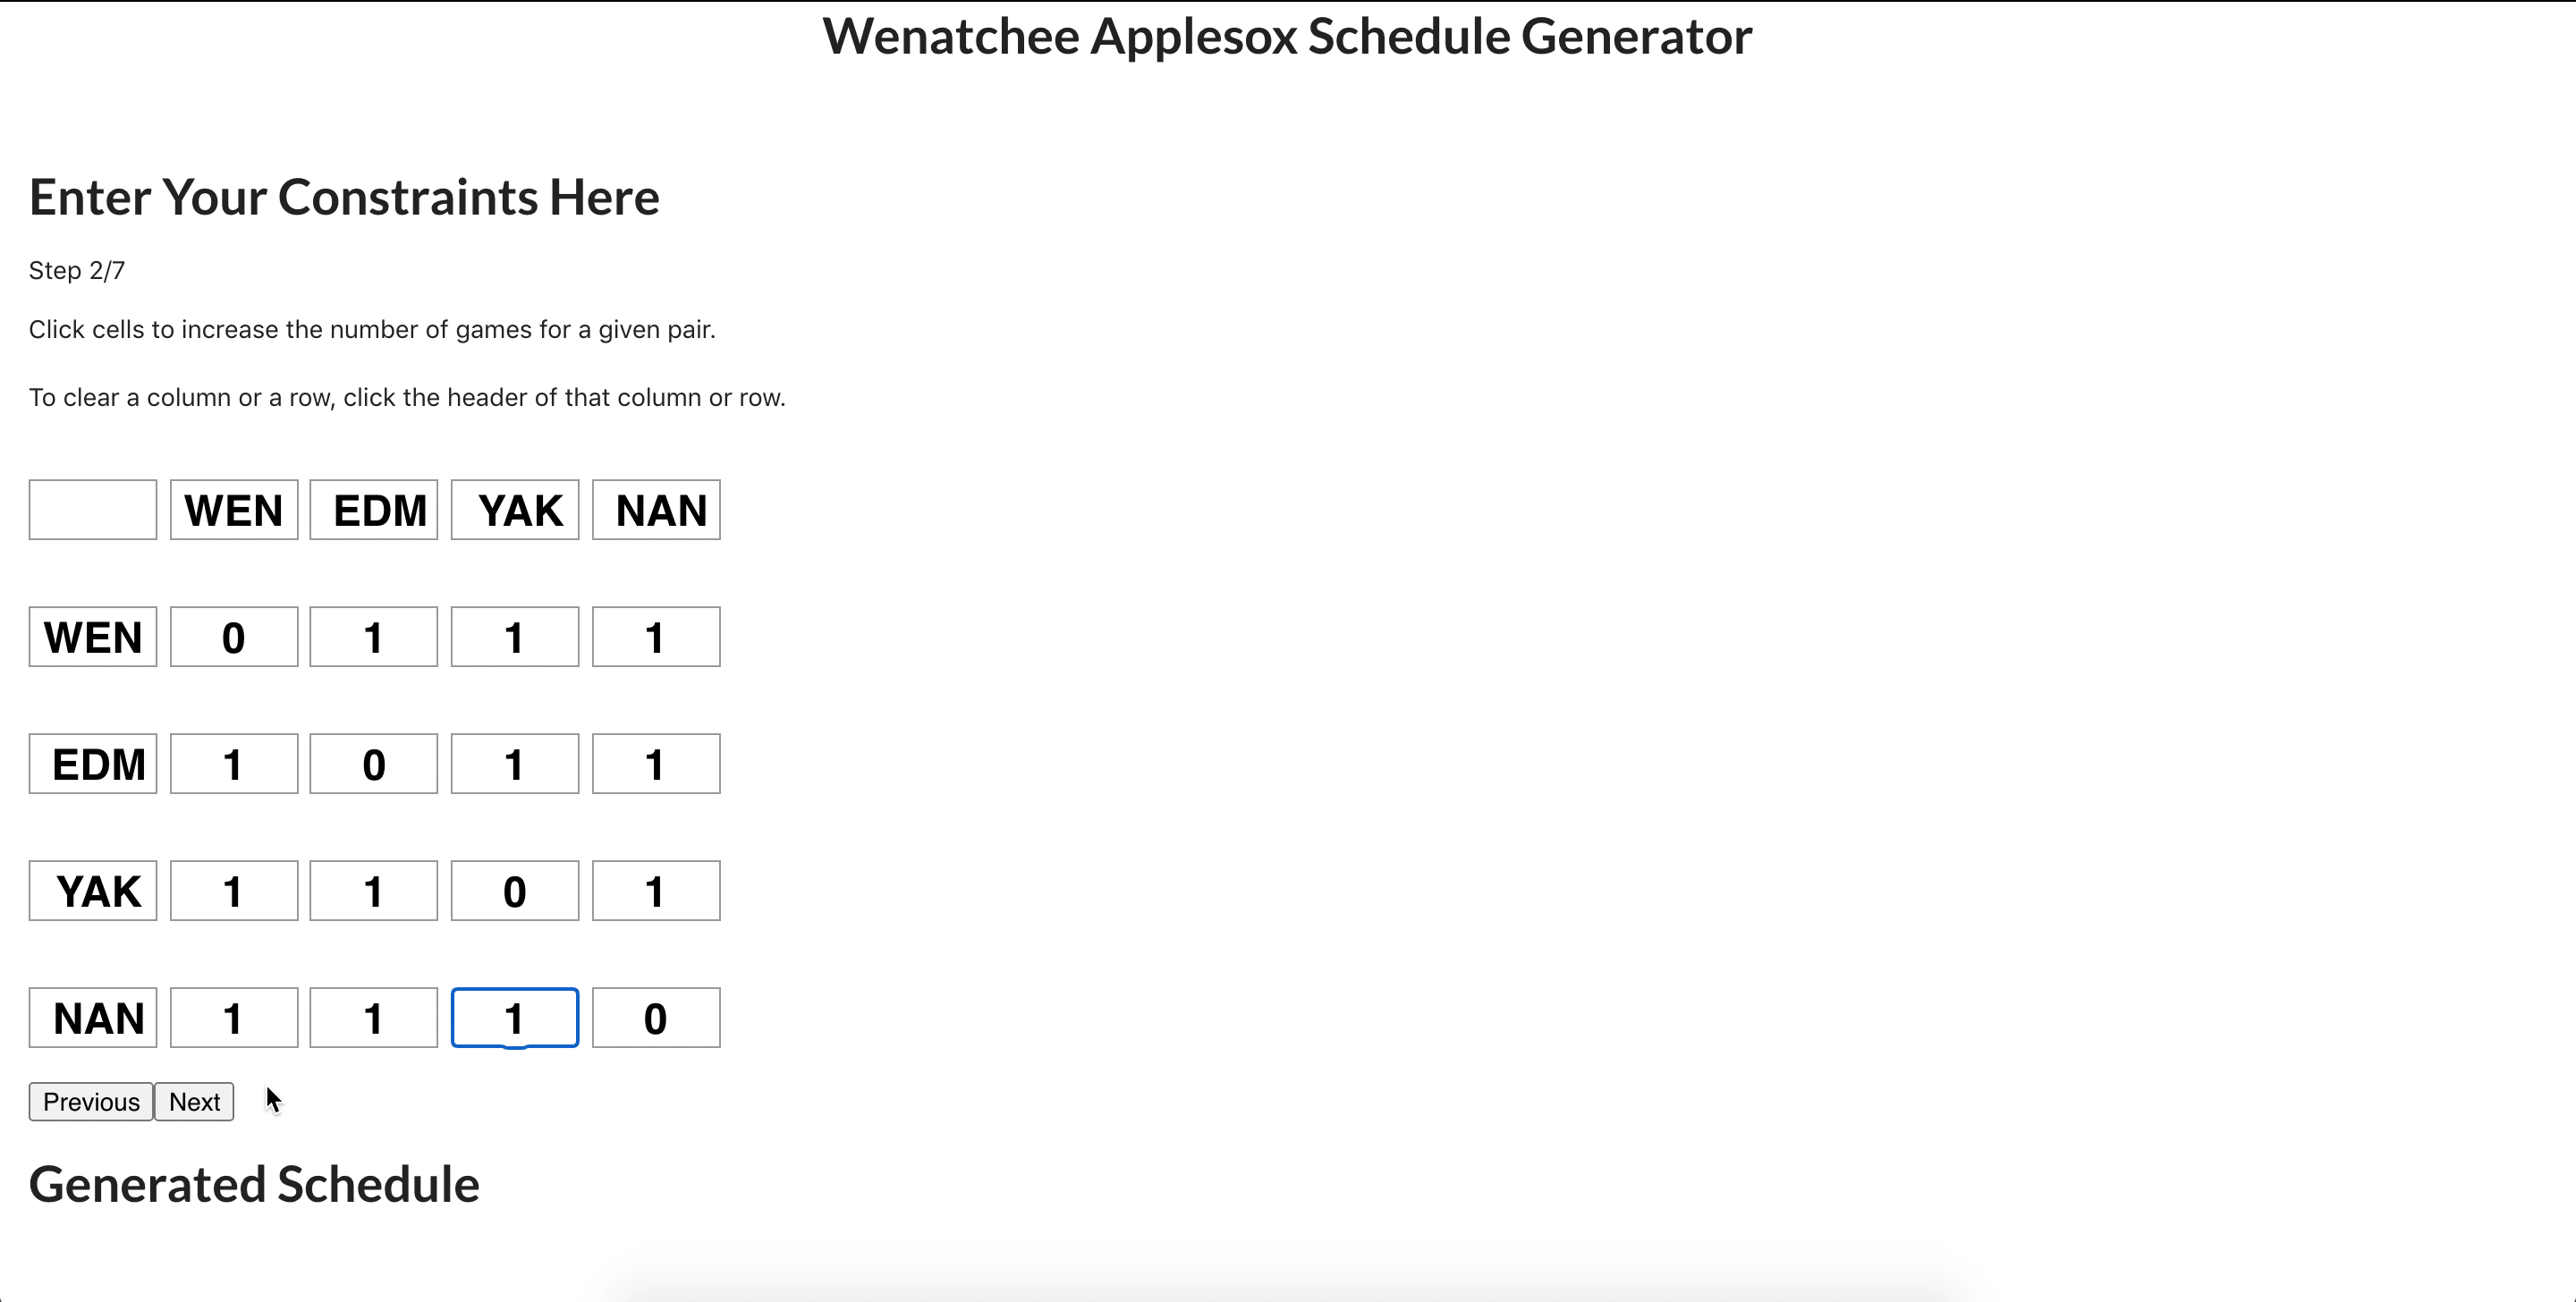
\includegraphics[scale=0.16]{Screen Shot 2021-05-07 at 1.27.57 AM.png}}  
    \caption{Step 2 of Input Form - Who Plays Who Matrix}
\end{figure}

\begin{figure}[h]
    \centering
    \fbox{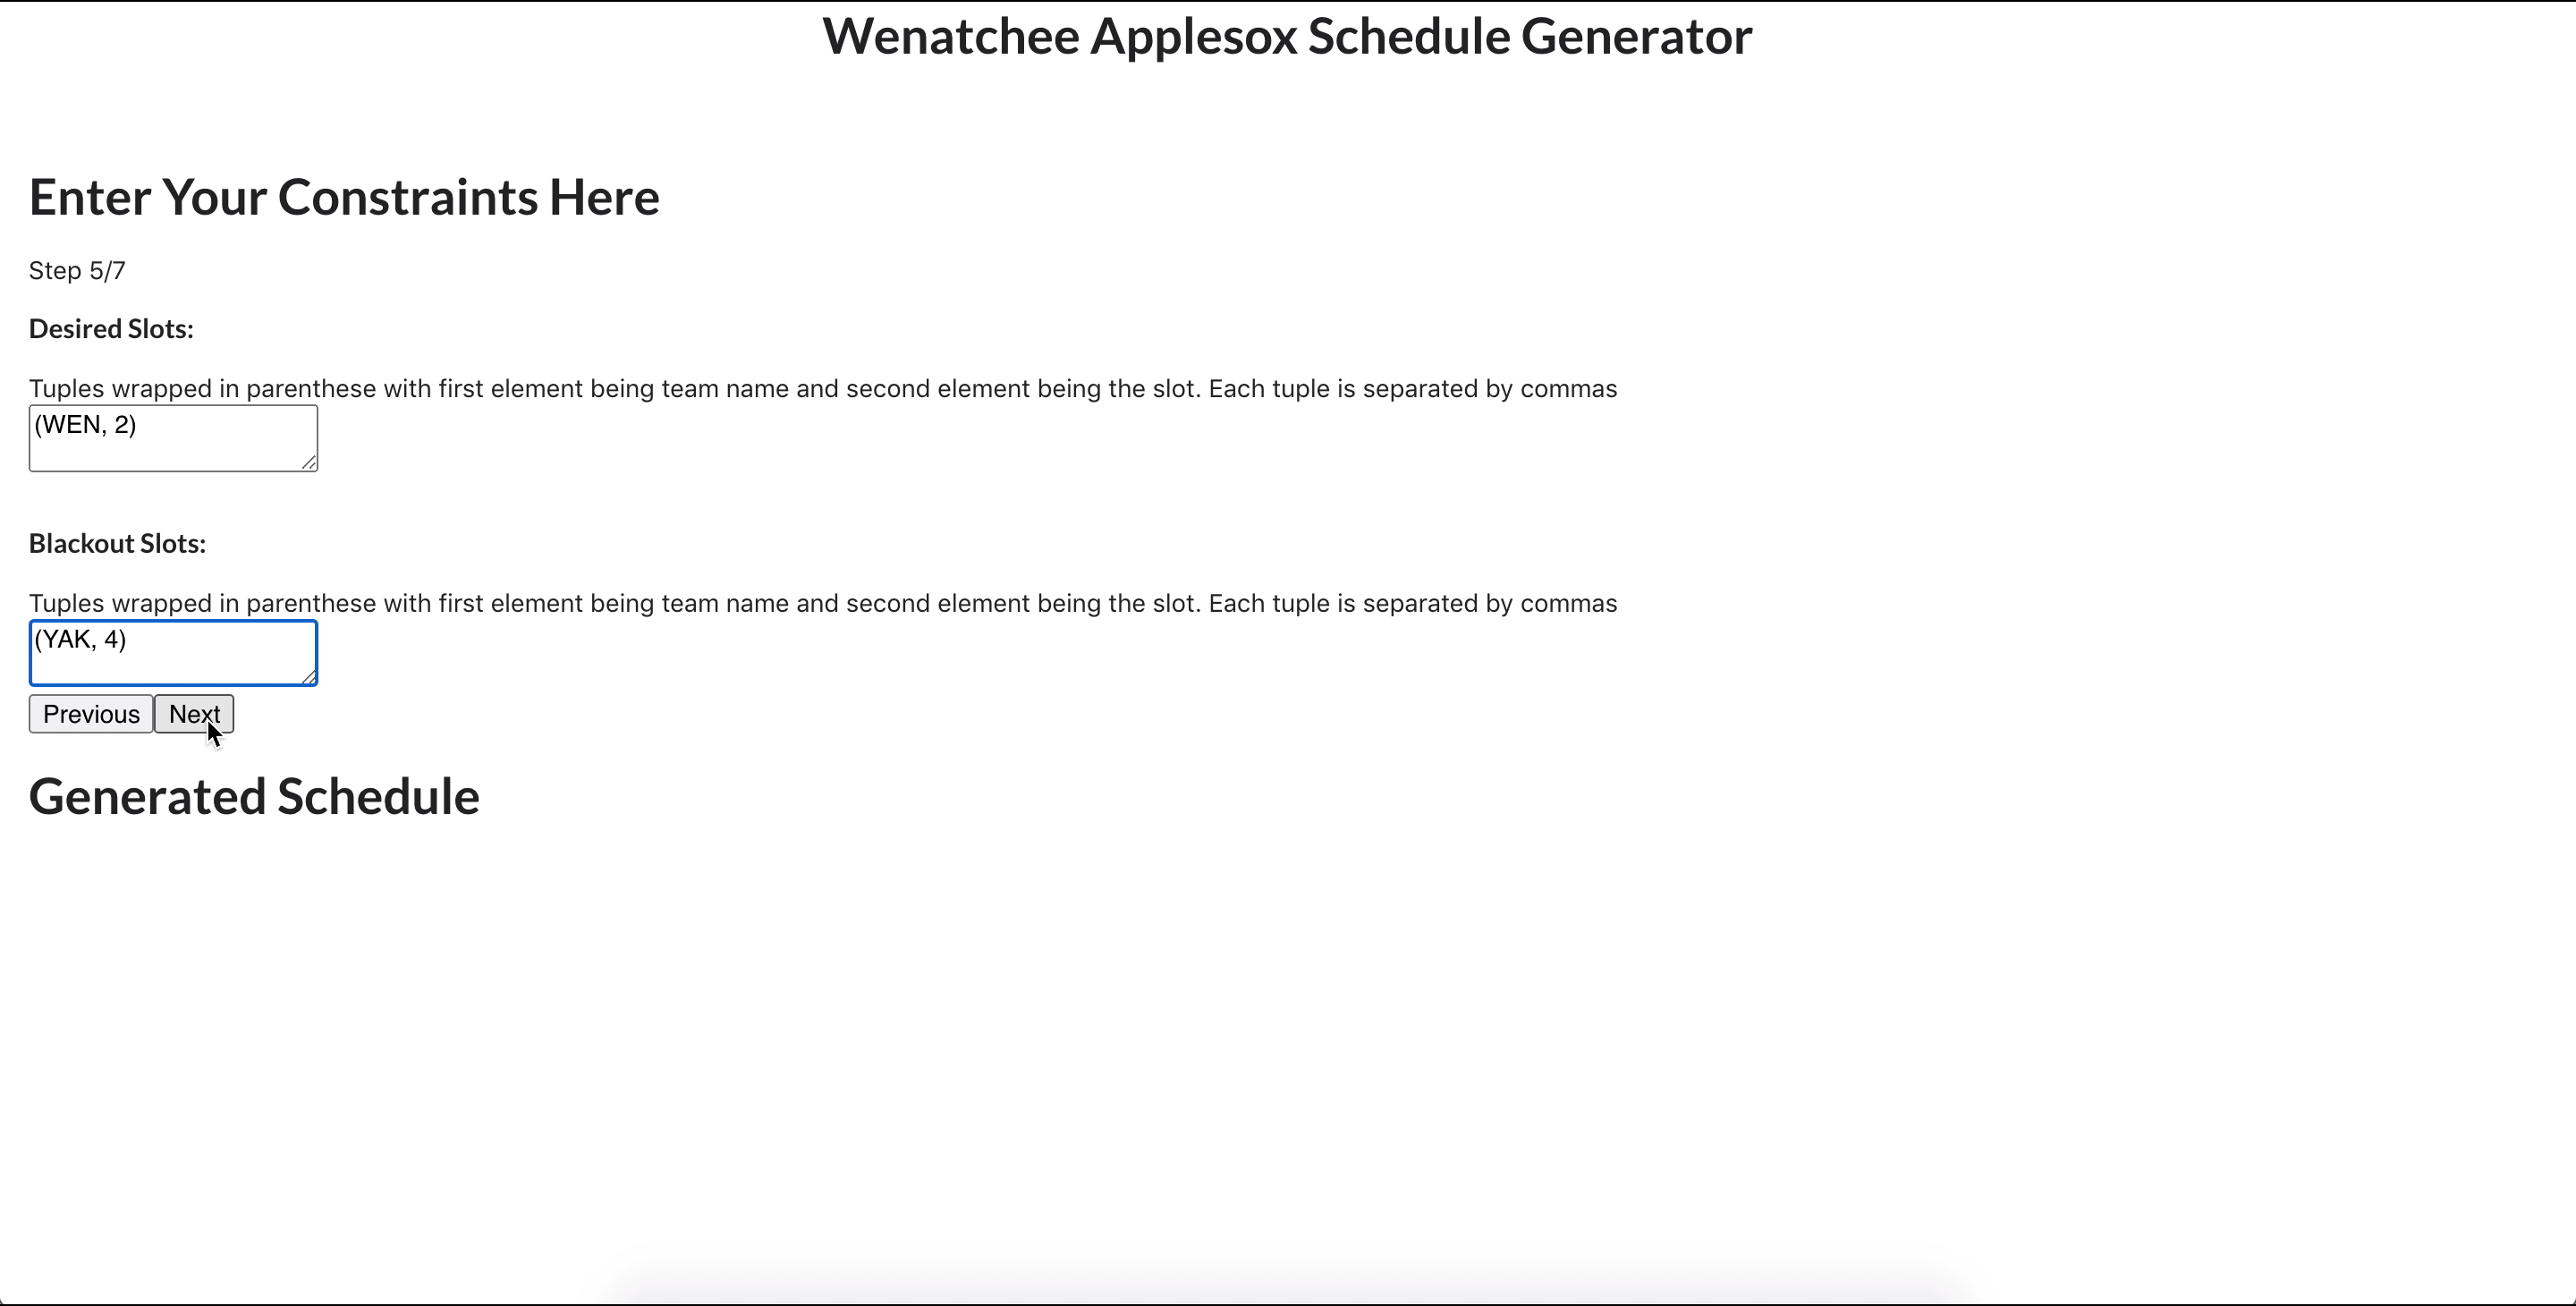
\includegraphics[scale=0.16]{Screen Shot 2021-05-07 at 1.28.43 AM.png}} 
    \caption{Step 5 of Input Form - Desired Slots & Blackout Slots}
\end{figure}

At the last page of inputs, a "Generate Schedule" button will appear on the bottom. In the case that an input value is missing or invalid, no schedule will be generated. Users will get a message that reads, "Schedule infeasible! Try changing your requirements." Else, when all of the inputs are valid to form a schedule, there will be a list of slots and games generated below. An example of that is shown in Figure 4.3 below. 


\begin{figure}[h]
    \centering
    \fbox{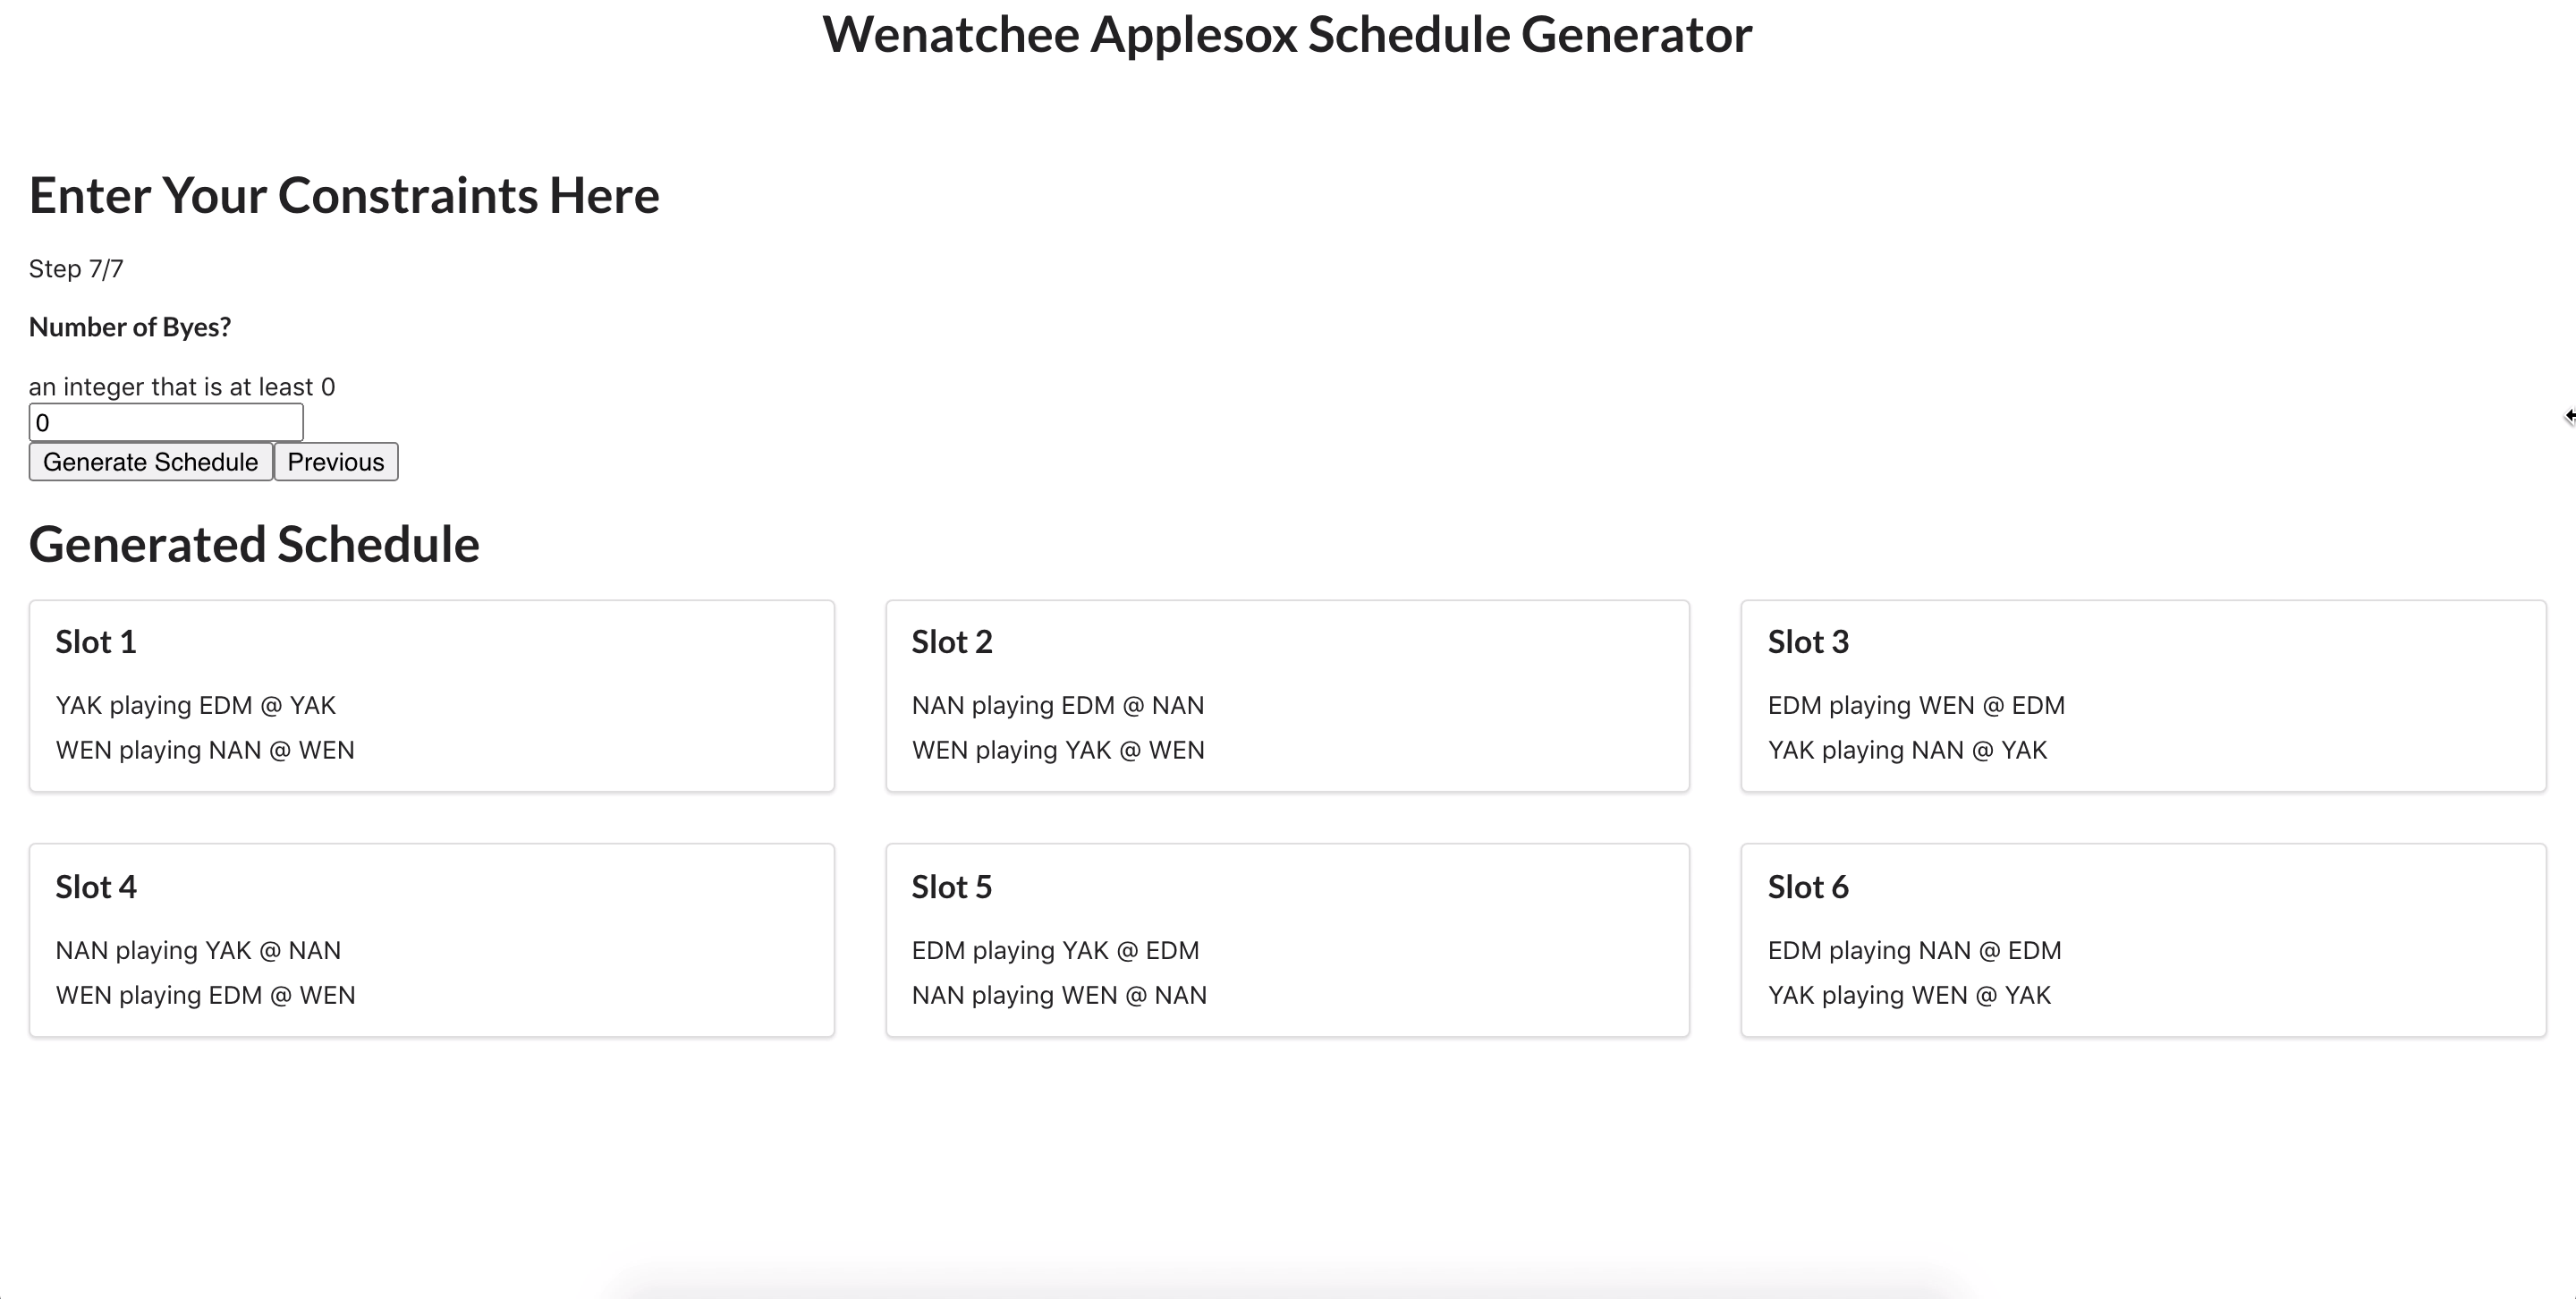
\includegraphics[scale=0.16]{Screen Shot 2021-05-07 at 1.29.06 AM.png}} 
    \caption{Step 7 of Input Form - Generated Schedule}
\end{figure}



\section{Command Line}
In addition to being able to run the solver via the web application, the solver can also be run via a command line tool. This tool allows the user to run generate schedules locally, without having to communicate with any servers. First, the user defines 3 files--a parameters file, a who plays who list file, and a cost matrix file--that will then be parsed by the command line tool and then sent to the solver in order to generate a schedule in Excel format.  

In order to run, the user enters the command \verb|python Scheduler.py -f| in the terminal and is then prompted to input the filenames of the input files as well as the filename of the generated schedule if the solver is able to find one. Note that the filenames must be entered with their extensions. To see all of the available commands for the scheduler, run the command \verb|python Scheduler.py -h|.



\section{Written Products}
Our liaison had also requested for us to make the process of how we made the solver well-documented and accessible to the public, in order to contribute to the open source community and to bring publicity to the West Coast League. Thus, we created two written documents that we hope will achieve that. The first is a report outlining the process of switching from the CPLEX ILP model to the open-source MIP package. We discuss the similarities and differences in the syntax of both, explaining how to "convert" from CPLEX into MIP. This document is included in Appendix C. We also discuss the accessibility and runtime of both. The second document is a Jupyter notebook, which is a format that allows us to embed runable code within a markdown text document. A PDF version of this notebook is included in Appendix A. In the notebook, we explain the different components of our main schedule solver file, walking the reader through how the code works and providing example schedule problems to solve. This makes it easy for the public to understand our code and add on or make changes to it to fit their needs. We plan on providing these documents to the liaisons for future distribution through a an open platform like Medium or through the League website. 

\chapter{Challenges}


\section{Optimizing for Travel}
Optimizing for travel was initially within the scope of the project, where our solver would output not just a valid schedule given the requirements, but the optimal schedule. But as we worked on modelling the problem as well as communicating with our liaison about the priorities and goals of the project, we realized that implementing travel optimization would be a significant undertaking, and that the feature was not worth the time and resources required, at least for this first iteration of the project.

Any optimization would depend heavily on the cost matrix given as input. The cost matrix simply defines the cost of travel between one team's home location to another team's home location--these are user-defined so that the user can account for not only miles but also difficulties in crossing boarders and typical traffic. We quickly realized that this was susceptible to both change and inaccuracy. While a solver could give the theoretical optimal schedule for a given cost matrix, parties from the league responsible for representing the teams and approving the schedule could have preferences not reflected in the cost matrix, or simply dislike the schedule presented. This pushed our approach more towards faster runtime, which allows us flexibility in generating and iterating on schedules, compared to the slower and more rigid schedules that an optimized solver would output.

On a high level, our model works by checking constraints for individual teams and slots. Optimizing for travel would require expanding our model to also check for relations between teams and games they play on consecutive slots and optimizing those. For $n$ teams in a league and $s$ slots for games in a season, the size of the matrix used in our current model is $N^2$ by $S$, as there are $n^2$ possible match ups between $n$ teams. Thus the size of the model is in $O(n^2)$

If we expanded the matrix to also be able to model the relations between consecutive matches, a lower bound on the size of the matrix would increase from $O(n^2)$ to $O(n^4)$. This is due to the fact that a variable modelling two consecutive games would have $n^2$ possible match ups for the first game, and $n^2$ possible match ups for the next. We can also think of this as adding an additional dimension to the matrix that we are solving, where the additional dimension is also of size $O(n^2)$.

While the runtime of our solver is not entirely dependent on the size of the matrix but also on the complexity of the constraints, our current implementation of the requirements iterate through all the variables in the matrix to add constraints, and so we are guaranteed to have an increase in runtime. The additional constraints regarding the actual optimization and consistency given the more complex model could make the runtime even worse. Adding all that to the actual work in formulating this expanded model and coding the constraints, our team decided to focus on other features. 

We are still able to optimize to some extent outside of the model by simply using random seeds, running the solver multiple times, and selecting the best schedule. It just does not find the optimal schedule. 



%%% Future Work
\chapter{Future Work}

\section{Known Bugs}
For the most part, we wanted to prioritize having an app that works in its entirety than an app that several incomplete features. By taking this approach, we sought to minimize the number of bugs in our code to provide the best user experience with what we have. That being said, there are still certain edge cases and abnormalities that do cause undesired behavior. 
For the web application, we trust that the user will input all of their requirements values in the same way that they are formatted in the examples both on the website and in other documentation. However, we do not preform any validation of the inputs upon receiving the values from the user. If the user were to put in undefined or unexpected parameters, the solver would not be able to handle these inputs.

A similar issue exists in the command line interface as well. The inputs need to be in a very specific format. No checks happen on the during the collection of these inputs. Unlike the web application, the command line interface fails rather silently. This makes debugging much more difficult as when the command line interface fails, it is unclear to the user what the issue might be. In the future, we would like to preform input validation for both interfaces and handle those errors in a clear, understandable way.

\section{Desired Features}
In the future, we would like to improve our project in a few ways. One would be to include travel optimization. As of right now, we do not account for travel in our scheduler. The addition of this optimization would allow for the creation of a schedule that takes into account the distance between the teams in the league as well. Another area to explore would be making our source code further open source to allow others to use our scheduler to create sports schedules for their leagues as well. This would help improve our own code and allow our work to be used by a greater audience. Lastly, we would like to invest further time into improving the UI of our web application. The current app's input form for parameters is simple and straightforward. It is such that users can use it easily, but it's not the most visually appeasing. There are many directions that this could go in, and it would be great to explore the different options to create the best UI experience for the app.  

In order to take on these challenges, it would help to look into a few specifics. One would be performing tests regarding the efficiency of the schedule generations, both the generated schedules and the solver run time. We did not have the opportunity to perform comparison tests to get statistics about the run time of our solvers. We think a good comparison point would be the schedules generated by the John Hopkins solver. Though we do not have access to the scheduler, we have access to the schedules generated for previous seasons, which we know to be pretty highly optimized. In addition to tests, further familiarization with MIP and its different settings with regards to how it approaches solving a model would allow for further optimization of our solver. Understanding the space complexity required for the constraints as well as the runtime complexity of solving the model in terms of constraints would be also be helpful on that front, as we have only done preliminary tests before moving onto other features for this project.

In order to include the travel optimization aforementioned, it could be useful to look into location APIs to automatically generate a rough cost matrix instead of requiring the user to input it as a parameter. Also, it would help to look into more React resources for development of the web application's UI. There are many useful, open-source React components that can be used to improve the fluidity of the input form components such as a calendar input which allows users to pull up a calendar to enter a date rather than a string. Digging around to see which React components can be used for the UI would improve the experience for users greatly. These are some of the initial starting points for completing the desired features. 

%%% Acknowledgements
\newpage
\textbf{Acknowledgements} \\
The Wenatchee AppleSox Clinic Team would like to thank our liaisons Jose Oglesby and Lauren Feaux and our project advisor Professor Boerkoel for their guidance and their contributions to the development process.


%%% For smaller documents---especially those you're writing by
%%% yourself---you might write your entire report using a single LaTeX
%%% source file.  For larger documents, we recommend that you split
%%% the source file into several separate, smaller files.  The smaller
%%% files are ``included'' into your main, or ``master'' document
%%% using \include commands.  See the template file for the Clinic
%%% reports for more details on how to split a LaTeX project into
%%% smaller files.


%%% The body of your Statement of Work should appear here.  See
%%% Chapter 4 in _The Mathematics Clinic in Brief: A Handbook_ for
%%% more details on what you should include in a Statement of Work.


%%% Appendices.

%%% For your Statement of Work, you probably won't have any
%%% appendices, but you could include some if you really needed to.

%%% The appendices are delineated with the \appendix command.
%%% Individual appendices are begun with the standard \chapter or
%%% \section commands.  In our example, we'll \include them just as we
%%% did other chapters.

%%% Even in a relatively short document such as your statement of
%%% work, you might need to have appendices.  If so, uncomment
%%% the \appendix command and add them below (remember, the
%%% top-level structural command in this format is section).

% \appendix
\appendix

\chapter{Jupyter Notebook for our Solver Class}
In  \href{https://colab.research.google.com/drive/140xD88TPd37yqrozWjob-Eaao1BY9Jgf?usp=sharing}{the Jupyter Notebook linked here}, we explain how our solver class works and include examples of how to use it. This is the underlying solver that creates schedules for both our command line and web app interfaces.


\chapter{Sample Excel Schedule}
% 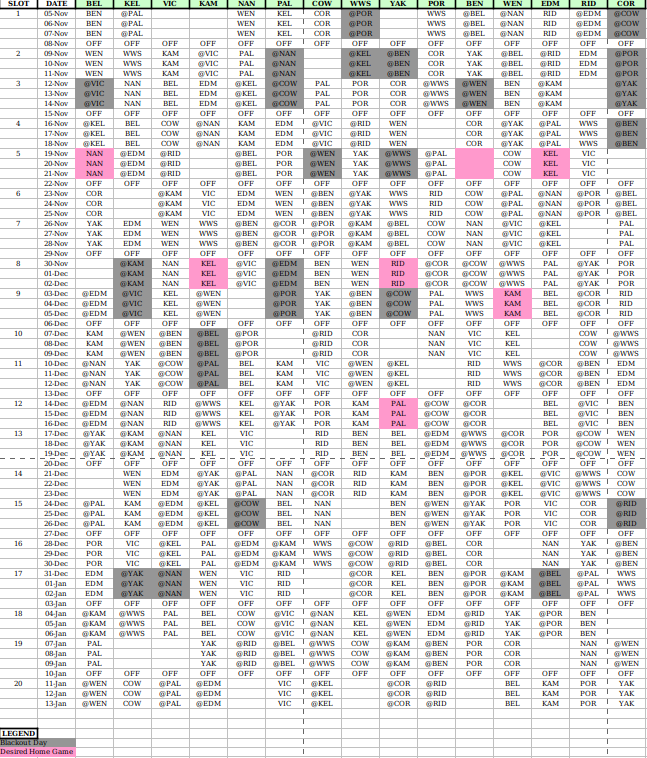
\includegraphics[scale=.6]{sample_excel_schedule.png}
% Table generated by Excel2LaTeX from sheet 'Sheet'
\begin{table}[htbp]
  \centering
  \tiny
  \tabcolsep=0.005cm
    \begin{tabular}{ccrrrrrrrrrrrrrrr}
    \toprule
    \multicolumn{1}{|c|}{\textbf{SLOT}} & \multicolumn{1}{c|}{\textbf{DATE}} & \multicolumn{1}{c|}{\cellcolor[rgb]{ .8,  1,  .8}\textbf{NAN}} & \multicolumn{1}{c|}{\cellcolor[rgb]{ .8,  1,  .8}\textbf{VIC}} & \multicolumn{1}{c|}{\cellcolor[rgb]{ .8,  1,  .8}\textbf{RID}} & \multicolumn{1}{c|}{\cellcolor[rgb]{ .8,  1,  .8}\textbf{EDM}} & \multicolumn{1}{c|}{\cellcolor[rgb]{ .8,  1,  .8}\textbf{PAL}} & \multicolumn{1}{c|}{\cellcolor[rgb]{ .8,  1,  .8}\textbf{WWS}} & \multicolumn{1}{c|}{\cellcolor[rgb]{ .8,  1,  .8}\textbf{POR}} & \multicolumn{1}{c|}{\cellcolor[rgb]{ .8,  1,  .8}\textbf{KAM}} & \multicolumn{1}{c|}{\cellcolor[rgb]{ .8,  1,  .8}\textbf{COR}} & \multicolumn{1}{c|}{\cellcolor[rgb]{ .8,  1,  .8}\textbf{YAK}} & \multicolumn{1}{c|}{\cellcolor[rgb]{ .8,  1,  .8}\textbf{BEL}} & \multicolumn{1}{c|}{\cellcolor[rgb]{ .8,  1,  .8}\textbf{COW}} & \multicolumn{1}{c|}{\cellcolor[rgb]{ .8,  1,  .8}\textbf{BEN}} & \multicolumn{1}{c|}{\cellcolor[rgb]{ .8,  1,  .8}\textbf{KEL}} & \multicolumn{1}{c|}{\cellcolor[rgb]{ .8,  1,  .8}\textbf{WEN}} \\
    \midrule
    1     & 05-Nov & \multicolumn{1}{c}{BEL} &       & \multicolumn{1}{c}{@POR} &       & \multicolumn{1}{c}{KAM} & \multicolumn{1}{c}{\cellcolor[rgb]{ .588,  .588,  .588}@KEL} & \multicolumn{1}{c}{RID} & \multicolumn{1}{c}{@PAL} & \multicolumn{1}{c}{\cellcolor[rgb]{ .588,  .588,  .588}@WEN} &       & \multicolumn{1}{c}{@NAN} & \multicolumn{1}{c}{BEN} & \multicolumn{1}{c}{@COW} & \multicolumn{1}{c}{WWS} & \multicolumn{1}{c}{COR} \\
          & 06-Nov & \multicolumn{1}{c}{BEL} &       & \multicolumn{1}{c}{@POR} &       & \multicolumn{1}{c}{KAM} & \multicolumn{1}{c}{\cellcolor[rgb]{ .588,  .588,  .588}@KEL} & \multicolumn{1}{c}{RID} & \multicolumn{1}{c}{@PAL} & \multicolumn{1}{c}{\cellcolor[rgb]{ .588,  .588,  .588}@WEN} &       & \multicolumn{1}{c}{@NAN} & \multicolumn{1}{c}{BEN} & \multicolumn{1}{c}{@COW} & \multicolumn{1}{c}{WWS} & \multicolumn{1}{c}{COR} \\
          & 07-Nov & \multicolumn{1}{c}{BEL} &       & \multicolumn{1}{c}{@POR} &       & \multicolumn{1}{c}{KAM} & \multicolumn{1}{c}{\cellcolor[rgb]{ .588,  .588,  .588}@KEL} & \multicolumn{1}{c}{RID} & \multicolumn{1}{c}{@PAL} & \multicolumn{1}{c}{\cellcolor[rgb]{ .588,  .588,  .588}@WEN} &       & \multicolumn{1}{c}{@NAN} & \multicolumn{1}{c}{BEN} & \multicolumn{1}{c}{@COW} & \multicolumn{1}{c}{WWS} & \multicolumn{1}{c}{COR} \\
          & 08-Nov & \multicolumn{1}{c}{OFF} & \multicolumn{1}{c}{OFF} & \multicolumn{1}{c}{OFF} & \multicolumn{1}{c}{OFF} & \multicolumn{1}{c}{OFF} & \multicolumn{1}{c}{OFF} & \multicolumn{1}{c}{OFF} & \multicolumn{1}{c}{OFF} & \multicolumn{1}{c}{OFF} & \multicolumn{1}{c}{OFF} & \multicolumn{1}{c}{OFF} & \multicolumn{1}{c}{OFF} & \multicolumn{1}{c}{OFF} & \multicolumn{1}{c}{OFF} & \multicolumn{1}{c}{OFF} \\
    2     & 09-Nov & \multicolumn{1}{c}{COW} & \multicolumn{1}{c}{@BEN} & \multicolumn{1}{c}{COR} & \multicolumn{1}{c}{POR} & \multicolumn{1}{c}{\cellcolor[rgb]{ .588,  .588,  .588}@KAM} & \multicolumn{1}{c}{\cellcolor[rgb]{ .588,  .588,  .588}@WEN} & \multicolumn{1}{c}{@EDM} & \multicolumn{1}{c}{PAL} & \multicolumn{1}{c}{\cellcolor[rgb]{ .588,  .588,  .588}@RID} & \multicolumn{1}{c}{\cellcolor[rgb]{ .588,  .588,  .588}@KEL} &       & \multicolumn{1}{c}{@NAN} & \multicolumn{1}{c}{VIC} & \multicolumn{1}{c}{YAK} & \multicolumn{1}{c}{WWS} \\
          & 10-Nov & \multicolumn{1}{c}{COW} & \multicolumn{1}{c}{@BEN} & \multicolumn{1}{c}{COR} & \multicolumn{1}{c}{POR} & \multicolumn{1}{c}{\cellcolor[rgb]{ .588,  .588,  .588}@KAM} & \multicolumn{1}{c}{\cellcolor[rgb]{ .588,  .588,  .588}@WEN} & \multicolumn{1}{c}{@EDM} & \multicolumn{1}{c}{PAL} & \multicolumn{1}{c}{\cellcolor[rgb]{ .588,  .588,  .588}@RID} & \multicolumn{1}{c}{\cellcolor[rgb]{ .588,  .588,  .588}@KEL} &       & \multicolumn{1}{c}{@NAN} & \multicolumn{1}{c}{VIC} & \multicolumn{1}{c}{YAK} & \multicolumn{1}{c}{WWS} \\
          & 11-Nov & \multicolumn{1}{c}{COW} & \multicolumn{1}{c}{@BEN} & \multicolumn{1}{c}{COR} & \multicolumn{1}{c}{POR} & \multicolumn{1}{c}{\cellcolor[rgb]{ .588,  .588,  .588}@KAM} & \multicolumn{1}{c}{\cellcolor[rgb]{ .588,  .588,  .588}@WEN} & \multicolumn{1}{c}{@EDM} & \multicolumn{1}{c}{PAL} & \multicolumn{1}{c}{\cellcolor[rgb]{ .588,  .588,  .588}@RID} & \multicolumn{1}{c}{\cellcolor[rgb]{ .588,  .588,  .588}@KEL} &       & \multicolumn{1}{c}{@NAN} & \multicolumn{1}{c}{VIC} & \multicolumn{1}{c}{YAK} & \multicolumn{1}{c}{WWS} \\
    3     & 12-Nov & \multicolumn{1}{c}{KAM} & \multicolumn{1}{c}{EDM} & \multicolumn{1}{c}{BEN} & \multicolumn{1}{c}{@VIC} & \multicolumn{1}{c}{\cellcolor[rgb]{ .588,  .588,  .588}@POR} &       & \multicolumn{1}{c}{PAL} & \multicolumn{1}{c}{@NAN} & \multicolumn{1}{c}{\cellcolor[rgb]{ .588,  .588,  .588}@COW} & \multicolumn{1}{c}{BEL} & \multicolumn{1}{c}{\cellcolor[rgb]{ .588,  .588,  .588}@YAK} & \multicolumn{1}{c}{COR} & \multicolumn{1}{c}{\cellcolor[rgb]{ .588,  .588,  .588}@RID} & \multicolumn{1}{c}{@WEN} & \multicolumn{1}{c}{KEL} \\
          & 13-Nov & \multicolumn{1}{c}{KAM} & \multicolumn{1}{c}{EDM} & \multicolumn{1}{c}{BEN} & \multicolumn{1}{c}{@VIC} & \multicolumn{1}{c}{\cellcolor[rgb]{ .588,  .588,  .588}@POR} &       & \multicolumn{1}{c}{PAL} & \multicolumn{1}{c}{@NAN} & \multicolumn{1}{c}{\cellcolor[rgb]{ .588,  .588,  .588}@COW} & \multicolumn{1}{c}{BEL} & \multicolumn{1}{c}{\cellcolor[rgb]{ .588,  .588,  .588}@YAK} & \multicolumn{1}{c}{COR} & \multicolumn{1}{c}{\cellcolor[rgb]{ .588,  .588,  .588}@RID} & \multicolumn{1}{c}{@WEN} & \multicolumn{1}{c}{KEL} \\
          & 14-Nov & \multicolumn{1}{c}{KAM} & \multicolumn{1}{c}{EDM} & \multicolumn{1}{c}{BEN} & \multicolumn{1}{c}{@VIC} & \multicolumn{1}{c}{\cellcolor[rgb]{ .588,  .588,  .588}@POR} &       & \multicolumn{1}{c}{PAL} & \multicolumn{1}{c}{@NAN} & \multicolumn{1}{c}{\cellcolor[rgb]{ .588,  .588,  .588}@COW} & \multicolumn{1}{c}{BEL} & \multicolumn{1}{c}{\cellcolor[rgb]{ .588,  .588,  .588}@YAK} & \multicolumn{1}{c}{COR} & \multicolumn{1}{c}{\cellcolor[rgb]{ .588,  .588,  .588}@RID} & \multicolumn{1}{c}{@WEN} & \multicolumn{1}{c}{KEL} \\
          & 15-Nov & \multicolumn{1}{c}{OFF} & \multicolumn{1}{c}{OFF} & \multicolumn{1}{c}{OFF} & \multicolumn{1}{c}{OFF} & \multicolumn{1}{c}{OFF} & \multicolumn{1}{c}{OFF} & \multicolumn{1}{c}{OFF} & \multicolumn{1}{c}{OFF} & \multicolumn{1}{c}{OFF} & \multicolumn{1}{c}{OFF} & \multicolumn{1}{c}{OFF} & \multicolumn{1}{c}{OFF} & \multicolumn{1}{c}{OFF} & \multicolumn{1}{c}{OFF} & \multicolumn{1}{c}{OFF} \\
    4     & 16-Nov & \multicolumn{1}{c}{@PAL} & \multicolumn{1}{c}{@COW} & \multicolumn{1}{c}{@EDM} & \multicolumn{1}{c}{RID} & \multicolumn{1}{c}{NAN} & \multicolumn{1}{c}{KEL} & \multicolumn{1}{c}{BEN} & \multicolumn{1}{c}{@WEN} & \multicolumn{1}{c}{\cellcolor[rgb]{ .588,  .588,  .588}@YAK} & \multicolumn{1}{c}{COR} &       & \multicolumn{1}{c}{VIC} & \multicolumn{1}{c}{@POR} & \multicolumn{1}{c}{@WWS} & \multicolumn{1}{c}{KAM} \\
          & 17-Nov & \multicolumn{1}{c}{@PAL} & \multicolumn{1}{c}{@COW} & \multicolumn{1}{c}{@EDM} & \multicolumn{1}{c}{RID} & \multicolumn{1}{c}{NAN} & \multicolumn{1}{c}{KEL} & \multicolumn{1}{c}{BEN} & \multicolumn{1}{c}{@WEN} & \multicolumn{1}{c}{\cellcolor[rgb]{ .588,  .588,  .588}@YAK} & \multicolumn{1}{c}{COR} &       & \multicolumn{1}{c}{VIC} & \multicolumn{1}{c}{@POR} & \multicolumn{1}{c}{@WWS} & \multicolumn{1}{c}{KAM} \\
          & 18-Nov & \multicolumn{1}{c}{@PAL} & \multicolumn{1}{c}{@COW} & \multicolumn{1}{c}{@EDM} & \multicolumn{1}{c}{RID} & \multicolumn{1}{c}{NAN} & \multicolumn{1}{c}{KEL} & \multicolumn{1}{c}{BEN} & \multicolumn{1}{c}{@WEN} & \multicolumn{1}{c}{\cellcolor[rgb]{ .588,  .588,  .588}@YAK} & \multicolumn{1}{c}{COR} &       & \multicolumn{1}{c}{VIC} & \multicolumn{1}{c}{@POR} & \multicolumn{1}{c}{@WWS} & \multicolumn{1}{c}{KAM} \\
    5     & 19-Nov & \multicolumn{1}{c}{KEL} & \multicolumn{1}{c}{@EDM} & \multicolumn{1}{c}{YAK} & \multicolumn{1}{c}{\cellcolor[rgb]{ 1,  .6,  .8}VIC} & \multicolumn{1}{c}{@BEL} & \multicolumn{1}{c}{COR} & \multicolumn{1}{c}{COW} & \multicolumn{1}{c}{WEN} & \multicolumn{1}{c}{@WWS} & \multicolumn{1}{c}{\cellcolor[rgb]{ .588,  .588,  .588}@RID} & \multicolumn{1}{c}{\cellcolor[rgb]{ 1,  .6,  .8}PAL} & \multicolumn{1}{c}{\cellcolor[rgb]{ .588,  .588,  .588}@POR} & \cellcolor[rgb]{ 1,  .6,  .8} & \multicolumn{1}{c}{@NAN} & \multicolumn{1}{c}{@KAM} \\
          & 20-Nov & \multicolumn{1}{c}{KEL} & \multicolumn{1}{c}{@EDM} & \multicolumn{1}{c}{YAK} & \multicolumn{1}{c}{\cellcolor[rgb]{ 1,  .6,  .8}VIC} & \multicolumn{1}{c}{@BEL} & \multicolumn{1}{c}{COR} & \multicolumn{1}{c}{COW} & \multicolumn{1}{c}{WEN} & \multicolumn{1}{c}{@WWS} & \multicolumn{1}{c}{\cellcolor[rgb]{ .588,  .588,  .588}@RID} & \multicolumn{1}{c}{\cellcolor[rgb]{ 1,  .6,  .8}PAL} & \multicolumn{1}{c}{\cellcolor[rgb]{ .588,  .588,  .588}@POR} & \cellcolor[rgb]{ 1,  .6,  .8} & \multicolumn{1}{c}{@NAN} & \multicolumn{1}{c}{@KAM} \\
          & 21-Nov & \multicolumn{1}{c}{KEL} & \multicolumn{1}{c}{@EDM} & \multicolumn{1}{c}{YAK} & \multicolumn{1}{c}{\cellcolor[rgb]{ 1,  .6,  .8}VIC} & \multicolumn{1}{c}{@BEL} & \multicolumn{1}{c}{COR} & \multicolumn{1}{c}{COW} & \multicolumn{1}{c}{WEN} & \multicolumn{1}{c}{@WWS} & \multicolumn{1}{c}{\cellcolor[rgb]{ .588,  .588,  .588}@RID} & \multicolumn{1}{c}{\cellcolor[rgb]{ 1,  .6,  .8}PAL} & \multicolumn{1}{c}{\cellcolor[rgb]{ .588,  .588,  .588}@POR} & \cellcolor[rgb]{ 1,  .6,  .8} & \multicolumn{1}{c}{@NAN} & \multicolumn{1}{c}{@KAM} \\
          & 22-Nov & \multicolumn{1}{c}{OFF} & \multicolumn{1}{c}{OFF} & \multicolumn{1}{c}{OFF} & \multicolumn{1}{c}{OFF} & \multicolumn{1}{c}{OFF} & \multicolumn{1}{c}{OFF} & \multicolumn{1}{c}{OFF} & \multicolumn{1}{c}{OFF} & \multicolumn{1}{c}{OFF} & \multicolumn{1}{c}{OFF} & \multicolumn{1}{c}{OFF} & \multicolumn{1}{c}{OFF} & \multicolumn{1}{c}{OFF} & \multicolumn{1}{c}{OFF} & \multicolumn{1}{c}{OFF} \\
    6     & 23-Nov & \multicolumn{1}{c}{VIC} & \multicolumn{1}{c}{@NAN} & \multicolumn{1}{c}{@PAL} &       & \multicolumn{1}{c}{RID} & \multicolumn{1}{c}{KAM} & \multicolumn{1}{c}{@COW} & \multicolumn{1}{c}{@WWS} &       & \multicolumn{1}{c}{KEL} & \multicolumn{1}{c}{WEN} & \multicolumn{1}{c}{POR} &       & \multicolumn{1}{c}{@YAK} & \multicolumn{1}{c}{@BEL} \\
          & 24-Nov & \multicolumn{1}{c}{VIC} & \multicolumn{1}{c}{@NAN} & \multicolumn{1}{c}{@PAL} &       & \multicolumn{1}{c}{RID} & \multicolumn{1}{c}{KAM} & \multicolumn{1}{c}{@COW} & \multicolumn{1}{c}{@WWS} &       & \multicolumn{1}{c}{KEL} & \multicolumn{1}{c}{WEN} & \multicolumn{1}{c}{POR} &       & \multicolumn{1}{c}{@YAK} & \multicolumn{1}{c}{@BEL} \\
          & 25-Nov & \multicolumn{1}{c}{VIC} & \multicolumn{1}{c}{@NAN} & \multicolumn{1}{c}{@PAL} &       & \multicolumn{1}{c}{RID} & \multicolumn{1}{c}{KAM} & \multicolumn{1}{c}{@COW} & \multicolumn{1}{c}{@WWS} &       & \multicolumn{1}{c}{KEL} & \multicolumn{1}{c}{WEN} & \multicolumn{1}{c}{POR} &       & \multicolumn{1}{c}{@YAK} & \multicolumn{1}{c}{@BEL} \\
    7     & 26-Nov & \multicolumn{1}{c}{@POR} & \multicolumn{1}{c}{COW} & \multicolumn{1}{c}{WWS} & \multicolumn{1}{c}{@KEL} &       & \multicolumn{1}{c}{@RID} & \multicolumn{1}{c}{NAN} & \multicolumn{1}{c}{BEL} &       &       & \multicolumn{1}{c}{@KAM} & \multicolumn{1}{c}{@VIC} & \multicolumn{1}{c}{@WEN} & \multicolumn{1}{c}{EDM} & \multicolumn{1}{c}{BEN} \\
          & 27-Nov & \multicolumn{1}{c}{@POR} & \multicolumn{1}{c}{COW} & \multicolumn{1}{c}{WWS} & \multicolumn{1}{c}{@KEL} &       & \multicolumn{1}{c}{@RID} & \multicolumn{1}{c}{NAN} & \multicolumn{1}{c}{BEL} &       &       & \multicolumn{1}{c}{@KAM} & \multicolumn{1}{c}{@VIC} & \multicolumn{1}{c}{@WEN} & \multicolumn{1}{c}{EDM} & \multicolumn{1}{c}{BEN} \\
          & 28-Nov & \multicolumn{1}{c}{@POR} & \multicolumn{1}{c}{COW} & \multicolumn{1}{c}{WWS} & \multicolumn{1}{c}{@KEL} &       & \multicolumn{1}{c}{@RID} & \multicolumn{1}{c}{NAN} & \multicolumn{1}{c}{BEL} &       &       & \multicolumn{1}{c}{@KAM} & \multicolumn{1}{c}{@VIC} & \multicolumn{1}{c}{@WEN} & \multicolumn{1}{c}{EDM} & \multicolumn{1}{c}{BEN} \\
          & 29-Nov & \multicolumn{1}{c}{OFF} & \multicolumn{1}{c}{OFF} & \multicolumn{1}{c}{OFF} & \multicolumn{1}{c}{OFF} & \multicolumn{1}{c}{OFF} & \multicolumn{1}{c}{OFF} & \multicolumn{1}{c}{OFF} & \multicolumn{1}{c}{OFF} & \multicolumn{1}{c}{OFF} & \multicolumn{1}{c}{OFF} & \multicolumn{1}{c}{OFF} & \multicolumn{1}{c}{OFF} & \multicolumn{1}{c}{OFF} & \multicolumn{1}{c}{OFF} & \multicolumn{1}{c}{OFF} \\
    8     & 30-Nov & \multicolumn{1}{c}{WEN} & \multicolumn{1}{c}{KEL} & \multicolumn{1}{c}{@YAK} & \multicolumn{1}{c}{BEL} & \multicolumn{1}{c}{\cellcolor[rgb]{ .588,  .588,  .588}@COW} & \multicolumn{1}{c}{@KAM} &       & \multicolumn{1}{c}{\cellcolor[rgb]{ 1,  .6,  .8}WWS} & \multicolumn{1}{c}{BEN} & \multicolumn{1}{c}{\cellcolor[rgb]{ 1,  .6,  .8}RID} & \multicolumn{1}{c}{@EDM} & \multicolumn{1}{c}{PAL} & \multicolumn{1}{c}{@COR} & \multicolumn{1}{c}{\cellcolor[rgb]{ .588,  .588,  .588}@VIC} & \multicolumn{1}{c}{@NAN} \\
          & 01-Dec & \multicolumn{1}{c}{WEN} & \multicolumn{1}{c}{KEL} & \multicolumn{1}{c}{@YAK} & \multicolumn{1}{c}{BEL} & \multicolumn{1}{c}{\cellcolor[rgb]{ .588,  .588,  .588}@COW} & \multicolumn{1}{c}{@KAM} &       & \multicolumn{1}{c}{\cellcolor[rgb]{ 1,  .6,  .8}WWS} & \multicolumn{1}{c}{BEN} & \multicolumn{1}{c}{\cellcolor[rgb]{ 1,  .6,  .8}RID} & \multicolumn{1}{c}{@EDM} & \multicolumn{1}{c}{PAL} & \multicolumn{1}{c}{@COR} & \multicolumn{1}{c}{\cellcolor[rgb]{ .588,  .588,  .588}@VIC} & \multicolumn{1}{c}{@NAN} \\
          & 02-Dec & \multicolumn{1}{c}{WEN} & \multicolumn{1}{c}{KEL} & \multicolumn{1}{c}{@YAK} & \multicolumn{1}{c}{BEL} & \multicolumn{1}{c}{\cellcolor[rgb]{ .588,  .588,  .588}@COW} & \multicolumn{1}{c}{@KAM} &       & \multicolumn{1}{c}{\cellcolor[rgb]{ 1,  .6,  .8}WWS} & \multicolumn{1}{c}{BEN} & \multicolumn{1}{c}{\cellcolor[rgb]{ 1,  .6,  .8}RID} & \multicolumn{1}{c}{@EDM} & \multicolumn{1}{c}{PAL} & \multicolumn{1}{c}{@COR} & \multicolumn{1}{c}{\cellcolor[rgb]{ .588,  .588,  .588}@VIC} & \multicolumn{1}{c}{@NAN} \\
    9     & 03-Dec & \multicolumn{1}{c}{PAL} & \multicolumn{1}{c}{@KAM} & \multicolumn{1}{c}{@COR} & \multicolumn{1}{c}{KEL} & \multicolumn{1}{c}{\cellcolor[rgb]{ .588,  .588,  .588}@NAN} & \multicolumn{1}{c}{YAK} & \multicolumn{1}{c}{@BEL} & \multicolumn{1}{c}{VIC} & \multicolumn{1}{c}{RID} & \multicolumn{1}{c}{\cellcolor[rgb]{ .588,  .588,  .588}@WWS} & \multicolumn{1}{c}{POR} & \multicolumn{1}{c}{@BEN} & \multicolumn{1}{c}{COW} & \multicolumn{1}{c}{\cellcolor[rgb]{ .588,  .588,  .588}@EDM} & \cellcolor[rgb]{ 1,  .6,  .8} \\
          & 04-Dec & \multicolumn{1}{c}{PAL} & \multicolumn{1}{c}{@KAM} & \multicolumn{1}{c}{@COR} & \multicolumn{1}{c}{KEL} & \multicolumn{1}{c}{\cellcolor[rgb]{ .588,  .588,  .588}@NAN} & \multicolumn{1}{c}{YAK} & \multicolumn{1}{c}{@BEL} & \multicolumn{1}{c}{VIC} & \multicolumn{1}{c}{RID} & \multicolumn{1}{c}{\cellcolor[rgb]{ .588,  .588,  .588}@WWS} & \multicolumn{1}{c}{POR} & \multicolumn{1}{c}{@BEN} & \multicolumn{1}{c}{COW} & \multicolumn{1}{c}{\cellcolor[rgb]{ .588,  .588,  .588}@EDM} & \cellcolor[rgb]{ 1,  .6,  .8} \\
          & 05-Dec & \multicolumn{1}{c}{PAL} & \multicolumn{1}{c}{@KAM} & \multicolumn{1}{c}{@COR} & \multicolumn{1}{c}{KEL} & \multicolumn{1}{c}{\cellcolor[rgb]{ .588,  .588,  .588}@NAN} & \multicolumn{1}{c}{YAK} & \multicolumn{1}{c}{@BEL} & \multicolumn{1}{c}{VIC} & \multicolumn{1}{c}{RID} & \multicolumn{1}{c}{\cellcolor[rgb]{ .588,  .588,  .588}@WWS} & \multicolumn{1}{c}{POR} & \multicolumn{1}{c}{@BEN} & \multicolumn{1}{c}{COW} & \multicolumn{1}{c}{\cellcolor[rgb]{ .588,  .588,  .588}@EDM} & \cellcolor[rgb]{ 1,  .6,  .8} \\
          & 06-Dec & \multicolumn{1}{c}{OFF} & \multicolumn{1}{c}{OFF} & \multicolumn{1}{c}{OFF} & \multicolumn{1}{c}{OFF} & \multicolumn{1}{c}{OFF} & \multicolumn{1}{c}{OFF} & \multicolumn{1}{c}{OFF} & \multicolumn{1}{c}{OFF} & \multicolumn{1}{c}{OFF} & \multicolumn{1}{c}{OFF} & \multicolumn{1}{c}{OFF} & \multicolumn{1}{c}{OFF} & \multicolumn{1}{c}{OFF} & \multicolumn{1}{c}{OFF} & \multicolumn{1}{c}{OFF} \\
    10    & 07-Dec & \multicolumn{1}{c}{@BEL} & \multicolumn{1}{c}{KAM} & \multicolumn{1}{c}{@WWS} & \multicolumn{1}{c}{@POR} & \multicolumn{1}{c}{WEN} & \multicolumn{1}{c}{RID} & \multicolumn{1}{c}{EDM} & \multicolumn{1}{c}{\cellcolor[rgb]{ .588,  .588,  .588}@VIC} & \multicolumn{1}{c}{@BEN} & \multicolumn{1}{c}{@COW} & \multicolumn{1}{c}{NAN} & \multicolumn{1}{c}{YAK} & \multicolumn{1}{c}{COR} &       & \multicolumn{1}{c}{@PAL} \\
          & 08-Dec & \multicolumn{1}{c}{@BEL} & \multicolumn{1}{c}{KAM} & \multicolumn{1}{c}{@WWS} & \multicolumn{1}{c}{@POR} & \multicolumn{1}{c}{WEN} & \multicolumn{1}{c}{RID} & \multicolumn{1}{c}{EDM} & \multicolumn{1}{c}{\cellcolor[rgb]{ .588,  .588,  .588}@VIC} & \multicolumn{1}{c}{@BEN} & \multicolumn{1}{c}{@COW} & \multicolumn{1}{c}{NAN} & \multicolumn{1}{c}{YAK} & \multicolumn{1}{c}{COR} &       & \multicolumn{1}{c}{@PAL} \\
          & 09-Dec & \multicolumn{1}{c}{@BEL} & \multicolumn{1}{c}{KAM} & \multicolumn{1}{c}{@WWS} & \multicolumn{1}{c}{@POR} & \multicolumn{1}{c}{WEN} & \multicolumn{1}{c}{RID} & \multicolumn{1}{c}{EDM} & \multicolumn{1}{c}{\cellcolor[rgb]{ .588,  .588,  .588}@VIC} & \multicolumn{1}{c}{@BEN} & \multicolumn{1}{c}{@COW} & \multicolumn{1}{c}{NAN} & \multicolumn{1}{c}{YAK} & \multicolumn{1}{c}{COR} &       & \multicolumn{1}{c}{@PAL} \\
    11    & 10-Dec & \multicolumn{1}{c}{@EDM} &       & \multicolumn{1}{c}{COW} & \multicolumn{1}{c}{NAN} &       & \multicolumn{1}{c}{@BEN} & \multicolumn{1}{c}{@COR} & \multicolumn{1}{c}{\cellcolor[rgb]{ .588,  .588,  .588}@BEL} & \multicolumn{1}{c}{POR} & \multicolumn{1}{c}{WEN} & \multicolumn{1}{c}{KAM} & \multicolumn{1}{c}{@RID} & \multicolumn{1}{c}{WWS} &       & \multicolumn{1}{c}{@YAK} \\
          & 11-Dec & \multicolumn{1}{c}{@EDM} &       & \multicolumn{1}{c}{COW} & \multicolumn{1}{c}{NAN} &       & \multicolumn{1}{c}{@BEN} & \multicolumn{1}{c}{@COR} & \multicolumn{1}{c}{\cellcolor[rgb]{ .588,  .588,  .588}@BEL} & \multicolumn{1}{c}{POR} & \multicolumn{1}{c}{WEN} & \multicolumn{1}{c}{KAM} & \multicolumn{1}{c}{@RID} & \multicolumn{1}{c}{WWS} &       & \multicolumn{1}{c}{@YAK} \\
          & 12-Dec & \multicolumn{1}{c}{@EDM} &       & \multicolumn{1}{c}{COW} & \multicolumn{1}{c}{NAN} &       & \multicolumn{1}{c}{@BEN} & \multicolumn{1}{c}{@COR} & \multicolumn{1}{c}{\cellcolor[rgb]{ .588,  .588,  .588}@BEL} & \multicolumn{1}{c}{POR} & \multicolumn{1}{c}{WEN} & \multicolumn{1}{c}{KAM} & \multicolumn{1}{c}{@RID} & \multicolumn{1}{c}{WWS} &       & \multicolumn{1}{c}{@YAK} \\
          & 13-Dec & \multicolumn{1}{c}{OFF} & \multicolumn{1}{c}{OFF} & \multicolumn{1}{c}{OFF} & \multicolumn{1}{c}{OFF} & \multicolumn{1}{c}{OFF} & \multicolumn{1}{c}{OFF} & \multicolumn{1}{c}{OFF} & \multicolumn{1}{c}{OFF} & \multicolumn{1}{c}{OFF} & \multicolumn{1}{c}{OFF} & \multicolumn{1}{c}{OFF} & \multicolumn{1}{c}{OFF} & \multicolumn{1}{c}{OFF} & \multicolumn{1}{c}{OFF} & \multicolumn{1}{c}{OFF} \\
    12    & 14-Dec &       & \multicolumn{1}{c}{@RID} & \multicolumn{1}{c}{VIC} & \multicolumn{1}{c}{@COR} & \multicolumn{1}{c}{BEL} & \multicolumn{1}{c}{@POR} & \multicolumn{1}{c}{WWS} & \multicolumn{1}{c}{KEL} & \multicolumn{1}{c}{EDM} & \multicolumn{1}{c}{\cellcolor[rgb]{ 1,  .6,  .8}BEN} & \multicolumn{1}{c}{@PAL} & \multicolumn{1}{c}{@WEN} & \multicolumn{1}{c}{@YAK} & \multicolumn{1}{c}{@KAM} & \multicolumn{1}{c}{COW} \\
          & 15-Dec &       & \multicolumn{1}{c}{@RID} & \multicolumn{1}{c}{VIC} & \multicolumn{1}{c}{@COR} & \multicolumn{1}{c}{BEL} & \multicolumn{1}{c}{@POR} & \multicolumn{1}{c}{WWS} & \multicolumn{1}{c}{KEL} & \multicolumn{1}{c}{EDM} & \multicolumn{1}{c}{\cellcolor[rgb]{ 1,  .6,  .8}BEN} & \multicolumn{1}{c}{@PAL} & \multicolumn{1}{c}{@WEN} & \multicolumn{1}{c}{@YAK} & \multicolumn{1}{c}{@KAM} & \multicolumn{1}{c}{COW} \\
          & 16-Dec &       & \multicolumn{1}{c}{@RID} & \multicolumn{1}{c}{VIC} & \multicolumn{1}{c}{@COR} & \multicolumn{1}{c}{BEL} & \multicolumn{1}{c}{@POR} & \multicolumn{1}{c}{WWS} & \multicolumn{1}{c}{KEL} & \multicolumn{1}{c}{EDM} & \multicolumn{1}{c}{\cellcolor[rgb]{ 1,  .6,  .8}BEN} & \multicolumn{1}{c}{@PAL} & \multicolumn{1}{c}{@WEN} & \multicolumn{1}{c}{@YAK} & \multicolumn{1}{c}{@KAM} & \multicolumn{1}{c}{COW} \\
    13    & 17-Dec &       & \multicolumn{1}{c}{WEN} & \multicolumn{1}{c}{@COW} & \multicolumn{1}{c}{@PAL} & \multicolumn{1}{c}{EDM} & \multicolumn{1}{c}{BEN} & \multicolumn{1}{c}{COR} & \multicolumn{1}{c}{KEL} & \multicolumn{1}{c}{@POR} & \multicolumn{1}{c}{@BEL} & \multicolumn{1}{c}{YAK} & \multicolumn{1}{c}{RID} & \multicolumn{1}{c}{@WWS} & \multicolumn{1}{c}{@KAM} & \multicolumn{1}{c}{@VIC} \\
          & 18-Dec &       & \multicolumn{1}{c}{WEN} & \multicolumn{1}{c}{@COW} & \multicolumn{1}{c}{@PAL} & \multicolumn{1}{c}{EDM} & \multicolumn{1}{c}{BEN} & \multicolumn{1}{c}{COR} & \multicolumn{1}{c}{KEL} & \multicolumn{1}{c}{@POR} & \multicolumn{1}{c}{@BEL} & \multicolumn{1}{c}{YAK} & \multicolumn{1}{c}{RID} & \multicolumn{1}{c}{@WWS} & \multicolumn{1}{c}{@KAM} & \multicolumn{1}{c}{@VIC} \\
          & 19-Dec &       & \multicolumn{1}{c}{WEN} & \multicolumn{1}{c}{@COW} & \multicolumn{1}{c}{@PAL} & \multicolumn{1}{c}{EDM} & \multicolumn{1}{c}{BEN} & \multicolumn{1}{c}{COR} & \multicolumn{1}{c}{KEL} & \multicolumn{1}{c}{@POR} & \multicolumn{1}{c}{@BEL} & \multicolumn{1}{c}{YAK} & \multicolumn{1}{c}{RID} & \multicolumn{1}{c}{@WWS} & \multicolumn{1}{c}{@KAM} & \multicolumn{1}{c}{@VIC} \\
          & 20-Dec & \multicolumn{1}{c}{OFF} & \multicolumn{1}{c}{OFF} & \multicolumn{1}{c}{OFF} & \multicolumn{1}{c}{OFF} & \multicolumn{1}{c}{OFF} & \multicolumn{1}{c}{OFF} & \multicolumn{1}{c}{OFF} & \multicolumn{1}{c}{OFF} & \multicolumn{1}{c}{OFF} & \multicolumn{1}{c}{OFF} & \multicolumn{1}{c}{OFF} & \multicolumn{1}{c}{OFF} & \multicolumn{1}{c}{OFF} & \multicolumn{1}{c}{OFF} & \multicolumn{1}{c}{OFF} \\
    14    & 21-Dec & \multicolumn{1}{c}{@VIC} & \multicolumn{1}{c}{NAN} & \multicolumn{1}{c}{POR} & \multicolumn{1}{c}{@KAM} & \multicolumn{1}{c}{@YAK} & \multicolumn{1}{c}{@COR} & \multicolumn{1}{c}{@RID} & \multicolumn{1}{c}{EDM} & \multicolumn{1}{c}{WWS} & \multicolumn{1}{c}{PAL} & \multicolumn{1}{c}{BEN} & \multicolumn{1}{c}{@KEL} & \multicolumn{1}{c}{@BEL} & \multicolumn{1}{c}{COW} &  \\
          & 22-Dec & \multicolumn{1}{c}{@VIC} & \multicolumn{1}{c}{NAN} & \multicolumn{1}{c}{POR} & \multicolumn{1}{c}{@KAM} & \multicolumn{1}{c}{@YAK} & \multicolumn{1}{c}{@COR} & \multicolumn{1}{c}{@RID} & \multicolumn{1}{c}{EDM} & \multicolumn{1}{c}{WWS} & \multicolumn{1}{c}{PAL} & \multicolumn{1}{c}{BEN} & \multicolumn{1}{c}{@KEL} & \multicolumn{1}{c}{@BEL} & \multicolumn{1}{c}{COW} &  \\
          & 23-Dec & \multicolumn{1}{c}{@VIC} & \multicolumn{1}{c}{NAN} & \multicolumn{1}{c}{POR} & \multicolumn{1}{c}{@KAM} & \multicolumn{1}{c}{@YAK} & \multicolumn{1}{c}{@COR} & \multicolumn{1}{c}{@RID} & \multicolumn{1}{c}{EDM} & \multicolumn{1}{c}{WWS} & \multicolumn{1}{c}{PAL} & \multicolumn{1}{c}{BEN} & \multicolumn{1}{c}{@KEL} & \multicolumn{1}{c}{@BEL} & \multicolumn{1}{c}{COW} &  \\
    15    & 24-Dec & \multicolumn{1}{c}{\cellcolor[rgb]{ .588,  .588,  .588}@BEN} & \multicolumn{1}{c}{PAL} & \multicolumn{1}{c}{EDM} & \multicolumn{1}{c}{@RID} & \multicolumn{1}{c}{@VIC} & \multicolumn{1}{c}{POR} & \multicolumn{1}{c}{@WWS} & \multicolumn{1}{c}{YAK} & \multicolumn{1}{c}{\cellcolor[rgb]{ .588,  .588,  .588}@BEL} & \multicolumn{1}{c}{@KAM} & \multicolumn{1}{c}{COR} &       & \multicolumn{1}{c}{NAN} & \multicolumn{1}{c}{WEN} & \multicolumn{1}{c}{@KEL} \\
          & 25-Dec & \multicolumn{1}{c}{\cellcolor[rgb]{ .588,  .588,  .588}@BEN} & \multicolumn{1}{c}{PAL} & \multicolumn{1}{c}{EDM} & \multicolumn{1}{c}{@RID} & \multicolumn{1}{c}{@VIC} & \multicolumn{1}{c}{POR} & \multicolumn{1}{c}{@WWS} & \multicolumn{1}{c}{YAK} & \multicolumn{1}{c}{\cellcolor[rgb]{ .588,  .588,  .588}@BEL} & \multicolumn{1}{c}{@KAM} & \multicolumn{1}{c}{COR} &       & \multicolumn{1}{c}{NAN} & \multicolumn{1}{c}{WEN} & \multicolumn{1}{c}{@KEL} \\
          & 26-Dec & \multicolumn{1}{c}{\cellcolor[rgb]{ .588,  .588,  .588}@BEN} & \multicolumn{1}{c}{PAL} & \multicolumn{1}{c}{EDM} & \multicolumn{1}{c}{@RID} & \multicolumn{1}{c}{@VIC} & \multicolumn{1}{c}{POR} & \multicolumn{1}{c}{@WWS} & \multicolumn{1}{c}{YAK} & \multicolumn{1}{c}{\cellcolor[rgb]{ .588,  .588,  .588}@BEL} & \multicolumn{1}{c}{@KAM} & \multicolumn{1}{c}{COR} &       & \multicolumn{1}{c}{NAN} & \multicolumn{1}{c}{WEN} & \multicolumn{1}{c}{@KEL} \\
          & 27-Dec & \multicolumn{1}{c}{OFF} & \multicolumn{1}{c}{OFF} & \multicolumn{1}{c}{OFF} & \multicolumn{1}{c}{OFF} & \multicolumn{1}{c}{OFF} & \multicolumn{1}{c}{OFF} & \multicolumn{1}{c}{OFF} & \multicolumn{1}{c}{OFF} & \multicolumn{1}{c}{OFF} & \multicolumn{1}{c}{OFF} & \multicolumn{1}{c}{OFF} & \multicolumn{1}{c}{OFF} & \multicolumn{1}{c}{OFF} & \multicolumn{1}{c}{OFF} & \multicolumn{1}{c}{OFF} \\
    16    & 28-Dec & \multicolumn{1}{c}{@COW} & \multicolumn{1}{c}{RID} & \multicolumn{1}{c}{@VIC} & \multicolumn{1}{c}{PAL} & \multicolumn{1}{c}{@EDM} &       & \multicolumn{1}{c}{BEN} & \multicolumn{1}{c}{@YAK} & \multicolumn{1}{c}{WEN} & \multicolumn{1}{c}{KAM} & \multicolumn{1}{c}{@KEL} & \multicolumn{1}{c}{NAN} & \multicolumn{1}{c}{@POR} & \multicolumn{1}{c}{BEL} & \multicolumn{1}{c}{@COR} \\
          & 29-Dec & \multicolumn{1}{c}{@COW} & \multicolumn{1}{c}{RID} & \multicolumn{1}{c}{@VIC} & \multicolumn{1}{c}{PAL} & \multicolumn{1}{c}{@EDM} &       & \multicolumn{1}{c}{BEN} & \multicolumn{1}{c}{@YAK} & \multicolumn{1}{c}{WEN} & \multicolumn{1}{c}{KAM} & \multicolumn{1}{c}{@KEL} & \multicolumn{1}{c}{NAN} & \multicolumn{1}{c}{@POR} & \multicolumn{1}{c}{BEL} & \multicolumn{1}{c}{@COR} \\
          & 30-Dec & \multicolumn{1}{c}{@COW} & \multicolumn{1}{c}{RID} & \multicolumn{1}{c}{@VIC} & \multicolumn{1}{c}{PAL} & \multicolumn{1}{c}{@EDM} &       & \multicolumn{1}{c}{BEN} & \multicolumn{1}{c}{@YAK} & \multicolumn{1}{c}{WEN} & \multicolumn{1}{c}{KAM} & \multicolumn{1}{c}{@KEL} & \multicolumn{1}{c}{NAN} & \multicolumn{1}{c}{@POR} & \multicolumn{1}{c}{BEL} & \multicolumn{1}{c}{@COR} \\
    17    & 31-Dec & \multicolumn{1}{c}{VIC} & \multicolumn{1}{c}{\cellcolor[rgb]{ .588,  .588,  .588}@NAN} &       & \multicolumn{1}{c}{\cellcolor[rgb]{ .588,  .588,  .588}@BEL} & \multicolumn{1}{c}{KEL} & \multicolumn{1}{c}{WEN} &       &       & \multicolumn{1}{c}{COW} & \multicolumn{1}{c}{@BEN} & \multicolumn{1}{c}{EDM} & \multicolumn{1}{c}{@COR} & \multicolumn{1}{c}{YAK} & \multicolumn{1}{c}{\cellcolor[rgb]{ .588,  .588,  .588}@PAL} & \multicolumn{1}{c}{@WWS} \\
          & 01-Jan & \multicolumn{1}{c}{VIC} & \multicolumn{1}{c}{\cellcolor[rgb]{ .588,  .588,  .588}@NAN} &       & \multicolumn{1}{c}{\cellcolor[rgb]{ .588,  .588,  .588}@BEL} & \multicolumn{1}{c}{KEL} & \multicolumn{1}{c}{WEN} &       &       & \multicolumn{1}{c}{COW} & \multicolumn{1}{c}{@BEN} & \multicolumn{1}{c}{EDM} & \multicolumn{1}{c}{@COR} & \multicolumn{1}{c}{YAK} & \multicolumn{1}{c}{\cellcolor[rgb]{ .588,  .588,  .588}@PAL} & \multicolumn{1}{c}{@WWS} \\
          & 02-Jan & \multicolumn{1}{c}{VIC} & \multicolumn{1}{c}{\cellcolor[rgb]{ .588,  .588,  .588}@NAN} &       & \multicolumn{1}{c}{\cellcolor[rgb]{ .588,  .588,  .588}@BEL} & \multicolumn{1}{c}{KEL} & \multicolumn{1}{c}{WEN} &       &       & \multicolumn{1}{c}{COW} & \multicolumn{1}{c}{@BEN} & \multicolumn{1}{c}{EDM} & \multicolumn{1}{c}{@COR} & \multicolumn{1}{c}{YAK} & \multicolumn{1}{c}{\cellcolor[rgb]{ .588,  .588,  .588}@PAL} & \multicolumn{1}{c}{@WWS} \\
          & 03-Jan & \multicolumn{1}{c}{OFF} & \multicolumn{1}{c}{OFF} & \multicolumn{1}{c}{OFF} & \multicolumn{1}{c}{OFF} & \multicolumn{1}{c}{OFF} & \multicolumn{1}{c}{OFF} & \multicolumn{1}{c}{OFF} & \multicolumn{1}{c}{OFF} & \multicolumn{1}{c}{OFF} & \multicolumn{1}{c}{OFF} & \multicolumn{1}{c}{OFF} & \multicolumn{1}{c}{OFF} & \multicolumn{1}{c}{OFF} & \multicolumn{1}{c}{OFF} & \multicolumn{1}{c}{OFF} \\
    18    & 04-Jan & \multicolumn{1}{c}{EDM} & \multicolumn{1}{c}{@PAL} &       & \multicolumn{1}{c}{@NAN} & \multicolumn{1}{c}{VIC} & \multicolumn{1}{c}{@COW} & \multicolumn{1}{c}{@BEN} & \multicolumn{1}{c}{@KEL} & \multicolumn{1}{c}{YAK} & \multicolumn{1}{c}{@COR} & \multicolumn{1}{c}{@WEN} & \multicolumn{1}{c}{WWS} & \multicolumn{1}{c}{POR} & \multicolumn{1}{c}{KAM} & \multicolumn{1}{c}{BEL} \\
          & 05-Jan & \multicolumn{1}{c}{EDM} & \multicolumn{1}{c}{@PAL} &       & \multicolumn{1}{c}{@NAN} & \multicolumn{1}{c}{VIC} & \multicolumn{1}{c}{@COW} & \multicolumn{1}{c}{@BEN} & \multicolumn{1}{c}{@KEL} & \multicolumn{1}{c}{YAK} & \multicolumn{1}{c}{@COR} & \multicolumn{1}{c}{@WEN} & \multicolumn{1}{c}{WWS} & \multicolumn{1}{c}{POR} & \multicolumn{1}{c}{KAM} & \multicolumn{1}{c}{BEL} \\
          & 06-Jan & \multicolumn{1}{c}{EDM} & \multicolumn{1}{c}{@PAL} &       & \multicolumn{1}{c}{@NAN} & \multicolumn{1}{c}{VIC} & \multicolumn{1}{c}{@COW} & \multicolumn{1}{c}{@BEN} & \multicolumn{1}{c}{@KEL} & \multicolumn{1}{c}{YAK} & \multicolumn{1}{c}{@COR} & \multicolumn{1}{c}{@WEN} & \multicolumn{1}{c}{WWS} & \multicolumn{1}{c}{POR} & \multicolumn{1}{c}{KAM} & \multicolumn{1}{c}{BEL} \\
    19    & 07-Jan & \multicolumn{1}{c}{@KEL} & \multicolumn{1}{c}{BEL} & \multicolumn{1}{c}{@BEN} & \multicolumn{1}{c}{KAM} & \multicolumn{1}{c}{@COR} & \multicolumn{1}{c}{@YAK} & \multicolumn{1}{c}{@WEN} & \multicolumn{1}{c}{@EDM} & \multicolumn{1}{c}{PAL} & \multicolumn{1}{c}{WWS} & \multicolumn{1}{c}{@VIC} &       & \multicolumn{1}{c}{RID} & \multicolumn{1}{c}{NAN} & \multicolumn{1}{c}{POR} \\
          & 08-Jan & \multicolumn{1}{c}{@KEL} & \multicolumn{1}{c}{BEL} & \multicolumn{1}{c}{@BEN} & \multicolumn{1}{c}{KAM} & \multicolumn{1}{c}{@COR} & \multicolumn{1}{c}{@YAK} & \multicolumn{1}{c}{@WEN} & \multicolumn{1}{c}{@EDM} & \multicolumn{1}{c}{PAL} & \multicolumn{1}{c}{WWS} & \multicolumn{1}{c}{@VIC} &       & \multicolumn{1}{c}{RID} & \multicolumn{1}{c}{NAN} & \multicolumn{1}{c}{POR} \\
          & 09-Jan & \multicolumn{1}{c}{@KEL} & \multicolumn{1}{c}{BEL} & \multicolumn{1}{c}{@BEN} & \multicolumn{1}{c}{KAM} & \multicolumn{1}{c}{@COR} & \multicolumn{1}{c}{@YAK} & \multicolumn{1}{c}{@WEN} & \multicolumn{1}{c}{@EDM} & \multicolumn{1}{c}{PAL} & \multicolumn{1}{c}{WWS} & \multicolumn{1}{c}{@VIC} &       & \multicolumn{1}{c}{RID} & \multicolumn{1}{c}{NAN} & \multicolumn{1}{c}{POR} \\
          & 10-Jan & \multicolumn{1}{c}{OFF} & \multicolumn{1}{c}{OFF} & \multicolumn{1}{c}{OFF} & \multicolumn{1}{c}{OFF} & \multicolumn{1}{c}{OFF} & \multicolumn{1}{c}{OFF} & \multicolumn{1}{c}{OFF} & \multicolumn{1}{c}{OFF} & \multicolumn{1}{c}{OFF} & \multicolumn{1}{c}{OFF} & \multicolumn{1}{c}{OFF} & \multicolumn{1}{c}{OFF} & \multicolumn{1}{c}{OFF} & \multicolumn{1}{c}{OFF} & \multicolumn{1}{c}{OFF} \\
    20    & 11-Jan & \multicolumn{1}{c}{@RID} & \multicolumn{1}{c}{@KEL} & \multicolumn{1}{c}{NAN} & \multicolumn{1}{c}{BEL} & \multicolumn{1}{c}{POR} & \multicolumn{1}{c}{COW} & \multicolumn{1}{c}{@PAL} &       & \multicolumn{1}{c}{@BEN} & \multicolumn{1}{c}{@WEN} & \multicolumn{1}{c}{@EDM} & \multicolumn{1}{c}{@WWS} & \multicolumn{1}{c}{COR} & \multicolumn{1}{c}{VIC} & \multicolumn{1}{c}{YAK} \\
          & 12-Jan & \multicolumn{1}{c}{@RID} & \multicolumn{1}{c}{@KEL} & \multicolumn{1}{c}{NAN} & \multicolumn{1}{c}{BEL} & \multicolumn{1}{c}{POR} & \multicolumn{1}{c}{COW} & \multicolumn{1}{c}{@PAL} &       & \multicolumn{1}{c}{@BEN} & \multicolumn{1}{c}{@WEN} & \multicolumn{1}{c}{@EDM} & \multicolumn{1}{c}{@WWS} & \multicolumn{1}{c}{COR} & \multicolumn{1}{c}{VIC} & \multicolumn{1}{c}{YAK} \\
          & 13-Jan & \multicolumn{1}{c}{@RID} & \multicolumn{1}{c}{@KEL} & \multicolumn{1}{c}{NAN} & \multicolumn{1}{c}{BEL} & \multicolumn{1}{c}{POR} & \multicolumn{1}{c}{COW} & \multicolumn{1}{c}{@PAL} &       & \multicolumn{1}{c}{@BEN} & \multicolumn{1}{c}{@WEN} & \multicolumn{1}{c}{@EDM} & \multicolumn{1}{c}{@WWS} & \multicolumn{1}{c}{COR} & \multicolumn{1}{c}{VIC} & \multicolumn{1}{c}{YAK} \\
          &       &       &       &       &       &       &       &       &       &       &       &       &       &       &       &  \\
          &       &       &       &       &       &       &       &       &       &       &       &       &       &       &       &  \\
\cmidrule{1-1}    \multicolumn{1}{|c|}{\textbf{LEGEND}} &       &       &       &       &       &       &       &       &       &       &       &       &       &       &       &  \\
\cmidrule{1-1}    \rowcolor[rgb]{ .588,  .588,  .588} \multicolumn{2}{c}{Blackout Day} & \cellcolor[rgb]{ 1,  1,  1} & \cellcolor[rgb]{ 1,  1,  1} & \cellcolor[rgb]{ 1,  1,  1} & \cellcolor[rgb]{ 1,  1,  1} & \cellcolor[rgb]{ 1,  1,  1} & \cellcolor[rgb]{ 1,  1,  1} & \cellcolor[rgb]{ 1,  1,  1} & \cellcolor[rgb]{ 1,  1,  1} & \cellcolor[rgb]{ 1,  1,  1} & \cellcolor[rgb]{ 1,  1,  1} & \cellcolor[rgb]{ 1,  1,  1} & \cellcolor[rgb]{ 1,  1,  1} & \cellcolor[rgb]{ 1,  1,  1} & \cellcolor[rgb]{ 1,  1,  1} & \cellcolor[rgb]{ 1,  1,  1} \\
    \rowcolor[rgb]{ 1,  .6,  .8} \multicolumn{2}{c}{Desired Home Game} & \cellcolor[rgb]{ 1,  1,  1} & \cellcolor[rgb]{ 1,  1,  1} & \cellcolor[rgb]{ 1,  1,  1} & \cellcolor[rgb]{ 1,  1,  1} & \cellcolor[rgb]{ 1,  1,  1} & \cellcolor[rgb]{ 1,  1,  1} & \cellcolor[rgb]{ 1,  1,  1} & \cellcolor[rgb]{ 1,  1,  1} & \cellcolor[rgb]{ 1,  1,  1} & \cellcolor[rgb]{ 1,  1,  1} & \cellcolor[rgb]{ 1,  1,  1} & \cellcolor[rgb]{ 1,  1,  1} & \cellcolor[rgb]{ 1,  1,  1} & \cellcolor[rgb]{ 1,  1,  1} & \cellcolor[rgb]{ 1,  1,  1} \\
    \end{tabular}%
  \label{tab:addlabel}%
\end{table}%


\chapter{Switching from CPLEX to MIP}
This semester, the Wenatchee Applesox clinic team started with migrating the backend code from using CPLEX to instead use MIP, mixed integer linear programming. The main reasons as to why this decision was made was due to costs. As we were preparing for deployment, we ran into the problem of increased costs in terms of using CPLEX. The numbers were beyond our budget, and so we decided to explore different options. During this process, we looked into using Gurobi or Knuth but both had issues related to cost or scaling. Thus, we decided to move forward with MIP. What sets MIP apart from these other options is that it is open sourced, which comes with many different benefits. Our biggest concern of cost was no longer a worry with MIP. More importantly, open source programs allow for public collaboration such that they are improved continuously over time and are reliable due to large user bases. With that being said, MIP specifically met our needs due to its fast multi solving nature which was perfect for solving our sports scheduling problem. After making this decision, we spent the following weeks performing the migration.


Luckily, the migration process was more straightforward than expected. We changed the pre-existing solver code to be object oriented and translated our constraints to fit MIP. Let us take a look at an example of a constraint that was changed in this process. Figure C.1 is a snippet of one of the constraints we had for the CPLEX solver. This constraint ensures that each team only plays once and there are no duplicates. 

\begin{figure}[h]
    \centering
    \fbox{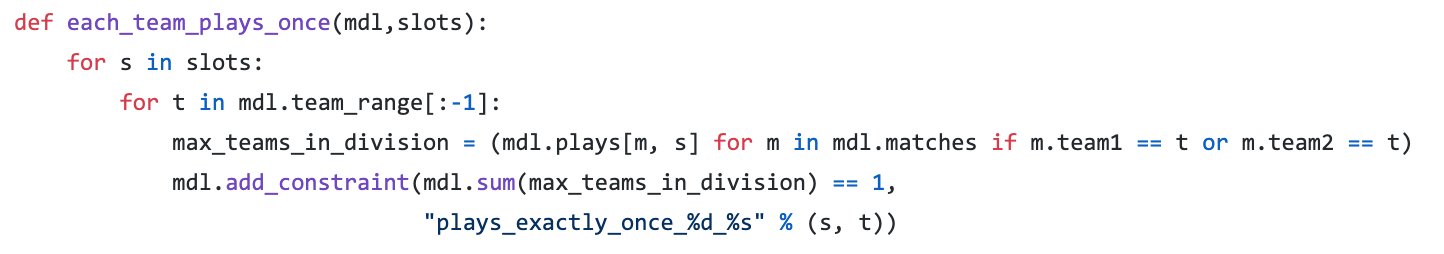
\includegraphics[scale=0.5]{Screen Shot 2021-03-01 at 2.39.57 PM.png}}  
    \caption{CPLEX Compatible “each\_team\_plays\_once” Implementation}
\end{figure}

Then, in comparison, we have Figure C.2, which is the new code that we have written this semester. The general structure of using the nested for loops to traverse through the slots is retained in this code. However, there are a few differences as well. First, we see that the MIP version of the code no longer takes in external parameters because self contains all of the needed information with object oriented code. Second, we utilize BYEs in this code to check whether a team is playing. Overall, due to the generally similar structure, the code translation process went smoothly. 

\begin{figure}[h]
    \centering
    \fbox{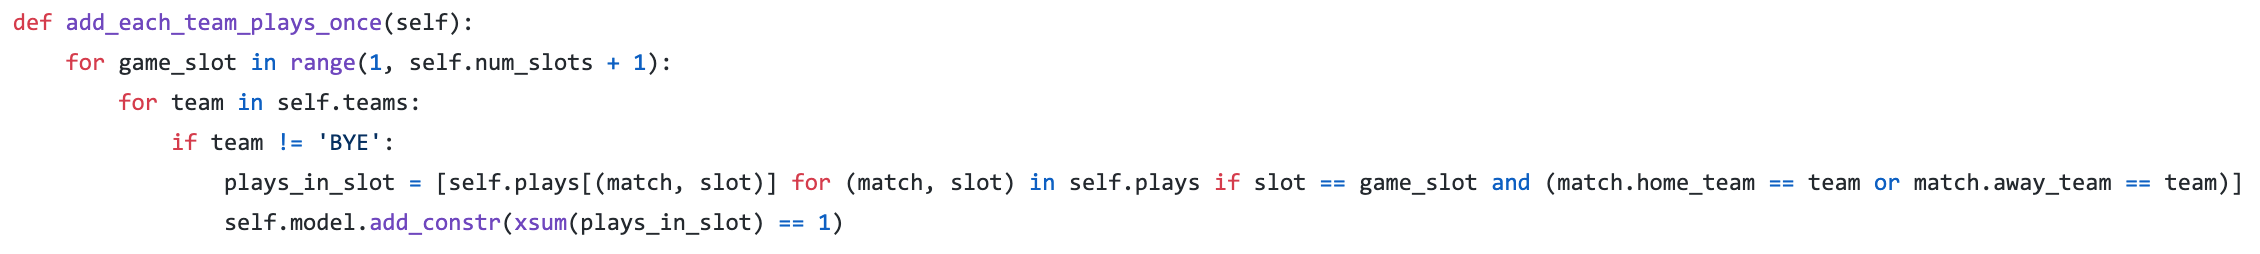
\includegraphics[scale=0.3]{Screen Shot 2021-03-01 at 2.41.07 PM.png}}  
    \caption{MIP Compatible “add\_each\_team\_plays\_once” Implementation}
\end{figure}


All of the translated code now resides in Scheduler.py with comments that detail each function and the general code itself. A lot of the translation process was aided by public resources from MIP and CPLEX. We now have a sport schedule solver that runs purely using MIP.



%%% Bibliography.

%%% BibTeX is the tool to use for citations and layout of your
%%% bibliography.  Instead of having to type ``[5]'' or ``(Jones,
%%% 1968)'' (and keep track of which citation is which and renumber
%%% them as you add more references to your bibilography), you use
%%% special commands that allow BibTeX and LaTeX to automatically put
%%% the correct information in the right place.

%%% Section 5.6 in _The Mathematics Clinic in Brief: A Handbook_,
%%% talks about using BibTeX to format your bibliography and
%%% citations.

%%% Depending on your field, it may or may not be appropriate to list
%%% references for which you haven't included specific citations.  If
%%% your field sanctions such practices, or if you just want to get an
%%% idea of what you have in your bibliography file, you can include
%%% everything with the \nocite{*} command.
\nocite{*} 


%%% The appearance of your bibliography and citations in your text are
%%% defined by a combination of any bibliography-related LaTeX
%%% packages (such as natbib, harvard, or chicago) and the particular
%%% bibliography style file that you load with the \bibliographystyle
%%% command.  Bibliography-style files end in .bst; you can find them
%%% by searching your file system using whatever tools you have for
%%% doing searches.  (On most modern Unices, ``locate .bst'' will give
%%% you an idea of what's available.)

\bibliographystyle{hmcmath}

%%% The particular bibliography data file or files that you want to
%%% use are specified with the \bibliography file.  Multiple files are
%%% separated by commas.

%%% You might want to use multiple bibliography (or ``bib'') files if
%%% you had a master bib file containing references you use again and
%%% again, and another containing only records for references for a
%%% particular project.
% https://www.overleaf.com/project/5c859a4520f6534f3c758817
%%% Many people create a single, large bib file that they use for
%%% everything they write.  That approach requires you to \cite every
%%% reference that you want to use in your document -- using
%%% \nocite{*} with a huge bibliography database will give you a large
%%% bibliography containing many references you haven't consulted for
%%% your particular document!

\bibliography{biblio}

%%% Glossary or Index.

%%% Having a glossary or index in a statement of work is overkill.
%%% Just define your terms in the text and you'll be fine.

\end{document}